\PassOptionsToPackage{unicode}{hyperref}
\PassOptionsToPackage{hyphens}{url}
\PassOptionsToPackage{dvipsnames,svgnames,x11names}{xcolor}
\documentclass[11pt]{article}

\usepackage{xcolor}
\usepackage[margin=1in]{geometry}
\usepackage{amsmath,amssymb}
\usepackage[T1]{fontenc}
\usepackage[utf8]{inputenc}
\usepackage{lmodern}
\usepackage{microtype}
\usepackage{setspace}
\usepackage{parskip}
\usepackage{longtable,booktabs,array,tabularx}
\usepackage{graphicx}
\usepackage{float}
\usepackage{pdflscape}
\usepackage{titling}
\usepackage{caption}
\usepackage{bookmark}
\usepackage[section]{placeins}
\usepackage{xurl}
\urlstyle{same}
\captionsetup{font=small,labelfont=bf}

\newcolumntype{Y}{>{\raggedright\arraybackslash}X}
\newcommand{\taxon}[1]{\emph{#1}}
\newcommand{\dcstsep}{/\allowbreak}
\newcounter{algorithm}
\newcommand{\algorithmtitle}[1]{%
  \refstepcounter{algorithm}%
  \noindent\textbf{Algorithm~\thealgorithm. #1}\par\nobreak\smallskip}
\newcommand{\paperaffiliation}{Center for Advanced Microbiome Research and Innovation (CAMRI), Institute for Genome Sciences, Department of Microbiology and Immunology, University of Maryland School of Medicine, Baltimore, Maryland, USA.}
\newcommand{\paperfundingnote}{Research reported in this publication was supported by grant number INV-048956 from the Gates Foundation.}
\newcommand{\blfootnote}[1]{%
  \begingroup
  \renewcommand{\thefootnote}{}\footnote{#1}%
  \addtocounter{footnote}{-1}%
  \endgroup}

\setlength{\droptitle}{-2.4em}
\pretitle{\begin{center}\Large}
\posttitle{\par\end{center}\vspace{0.55em}}
\preauthor{\begin{center}\normalsize}
\postauthor{\par\end{center}\vspace{-0.5em}}
\predate{}
\postdate{}

\hypersetup{
  pdftitle={Dominant-Community State Types Define a Deterministic Framework for Microbiome State Representation},
  colorlinks=true,
  linkcolor={blue},
  filecolor={Maroon},
  citecolor={Blue},
  urlcolor={blue},
  pdfcreator={LaTeX}}

\title{Dominant-Community State Types Define a Deterministic Framework for Microbiome State Representation}
\author{Pawel Gajer and Jacques Ravel}
\date{}
\newif\ifshowbuildstamp
\showbuildstampfalse
\providecommand{\manuscriptversion}{unversioned}
\providecommand{\manuscriptbuildnumber}{NA}
\providecommand{\manuscriptcommit}{unknown}
\providecommand{\manuscriptbuilddatetime}{unknown}
\InputIfFileExists{../build/manuscript_build_info.tex}{}{}

\begin{document}
\maketitle
\ifshowbuildstamp
\begin{center}
\footnotesize
Build: \manuscriptbuilddatetime
\end{center}
\vspace{0.35em}
\fi
\blfootnote{\paperaffiliation}
\blfootnote{\paperfundingnote}

\begin{abstract}
Microbiome state labels reduce high-dimensional abundance tables to ecological
summaries, but clustering-derived labels can drift with the comparison cohort,
distance metric, initialization, or number of clusters. We present
dominant-community state types (dCSTs), a deterministic rank-based framework in
which each sample has a dominance-lineage defined over a retained feature
family. Under the absorb policy used here, the fitted hierarchy is deterministic
for a fixed reference cohort, retained features, tie rule, and support schedule;
once frozen, it provides stable assignment for aligned cohorts.

We evaluate dCSTs in two microbiome settings. In gut data, a shared-taxonomy
American Gut Project dCST vocabulary transfers clinically coherent sample-level
IBD structure into external cohorts, especially Halfvarson 2017, while
subject-aware sensitivity bounds the portability claim. In vaginal metagenomes,
full-VOG dCSTs organize \textit{Chlamydia trachomatis} clearance and persistence
within the labeled CT cohort, with support from feature-cap robustness and
taxonomic, product-level, and KEGG-linked interpretation. Together, the two
applications use dCSTs as a deterministic state vocabulary for portability
analysis and local biological interpretation, not as a universal biomarker set.
\end{abstract}

\section{Introduction}

Microbiome studies often need a compact state language. Community-state types,
enterotypes, and related coarse labels turn high-dimensional abundance tables
into summaries that can be compared across samples, cohorts, and phenotypes
\cite{Ravel2011_CST,Gajer2012_CST,Arumugam2011_enterotypes}. However, many
widely used state labels are defined by clustering or other cohort-level
partitioning procedures, so the meaning of a label can shift with the comparison
cohort, distance metric, or partitioning rule. When the label itself drifts,
portability and reproducibility become harder to interpret.

This instability matters especially when the scientific question is not only
descriptive. External validation, transfer across cohorts, repeated-sample
sensitivity, and biological follow-up all benefit from labels that are defined
sample by sample rather than only relative to a fitted clustering solution. A
state label that changes when neighboring samples are added or removed is less
useful as a unit of biological comparison, and it is harder to treat as a
stable interface between microbiome measurements and downstream inference. For
that reason, there is value in microbiome-state labels built from a
deterministic assignment rule rather than a cluster membership produced by a
global optimization.

In contrast to clustering-defined CST or enterotype labels, which depend on a
clustering algorithm, distance metric, initialization, and number-of-clusters
parameter, an absorb-policy dCST label is determined by a retained feature
family, a deterministic tie rule, and a depth-specific support schedule. The
two fitted hierarchies analyzed in this paper give a sense of the resulting
scale (Table~\ref{tab:fitted-hierarchies}); the formal construction is given in
Methods~Section~\ref{sec:dcst-framework}.

This paper focuses on that representation problem. Existing state frameworks
are valuable when the goal is to discover clusters, fit mixture models, or
assign samples to a curated centroid vocabulary. dCSTs address a complementary
need: once a retained feature family and support policy have been specified,
they define rank-based sample states that can be named, frozen, transferred,
rebuilt, and tested without refitting a distance-based partition.

\begin{table}[!t]
\centering
\footnotesize
\setlength{\tabcolsep}{5pt}
\renewcommand{\arraystretch}{1.15}
\begin{tabular}{@{} l r r r r r r r @{}}
\toprule
 & & & & \multicolumn{4}{c}{Retained dCST states} \\
\cmidrule(lr){5-8}
Application & Cohort $n$ & Outcome subset $n$ & Features in $\mathcal{F}$ & $\ell{=}1$ & $\ell{=}2$ & $\ell{=}3$ & $\ell{=}4$ \\
\midrule
Gut (AGP, taxa) & 24,421 & 24,421 & 340 & 50 & 158 & 219 & 221 \\
CT (full-VOG)   & 3,602  & 604    & 509,501 & 12 & 23 & 52 & 68 \\
\bottomrule
\end{tabular}
\caption{Fitted dCST hierarchies analyzed in this paper. Cohort $n$ is the
structure-learning cohort used to fit the absorb-policy hierarchy; outcome
subset $n$ is the labeled subset on which outcome contrasts are evaluated
(identical to the structure-learning cohort in gut, restricted to the labeled
604 metagenomes in CT). Retained-state counts at depth $\ell$ are after
absorb-policy reassignment under the support schedules listed in
Supplementary Table~S2.}
\label{tab:fitted-hierarchies}
\end{table}

Dominant-community state types (dCSTs) were developed for this purpose. A
pre-policy dCST lineage is a rank-based dominance path built from a retained
feature family: samples are assigned first by their dominant retained feature
and then recursively refined by the next dominant retained feature within each
retained parent state. With the absorb policy used here, small provisional
child states are reassigned into nearby retained named states rather than
pooled into one residual bucket. The fitted absorb-policy vocabulary is
deterministic for a specified reference cohort, retained feature family, tie
rule, and support schedule; after freezing, it provides stable assignment into
explicit retained-feature lineages for aligned samples. The analyses that
follow focus on stability, transfer, and interpretation, not universal
biomarker discovery.

We evaluate dCSTs in two applications. The gut application tests portability:
whether a taxonomic dCST vocabulary learned in a large shared-taxonomy American
Gut Project background transfers into clinically annotated IBD cohorts, how
direct transfer compares with cohort-specific rebuilt hierarchies, and how
those signals behave under subject-aware sensitivity. The vaginal metagenomic
CT application tests within-cohort interpretation: whether the same
construction remains useful in a different niche and feature universe, using
full-VOG gene-family states with taxonomic, product-level, and KEGG-linked
follow-up. Together, the settings test whether dCSTs can provide deterministic,
interpretable state construction without clustering-defined labels;
cross-cohort portability under compatible conditions in gut IBD; and
within-cohort metagenomic interpretation in an independent CT setting.

\begin{figure}[H]
\centering
% 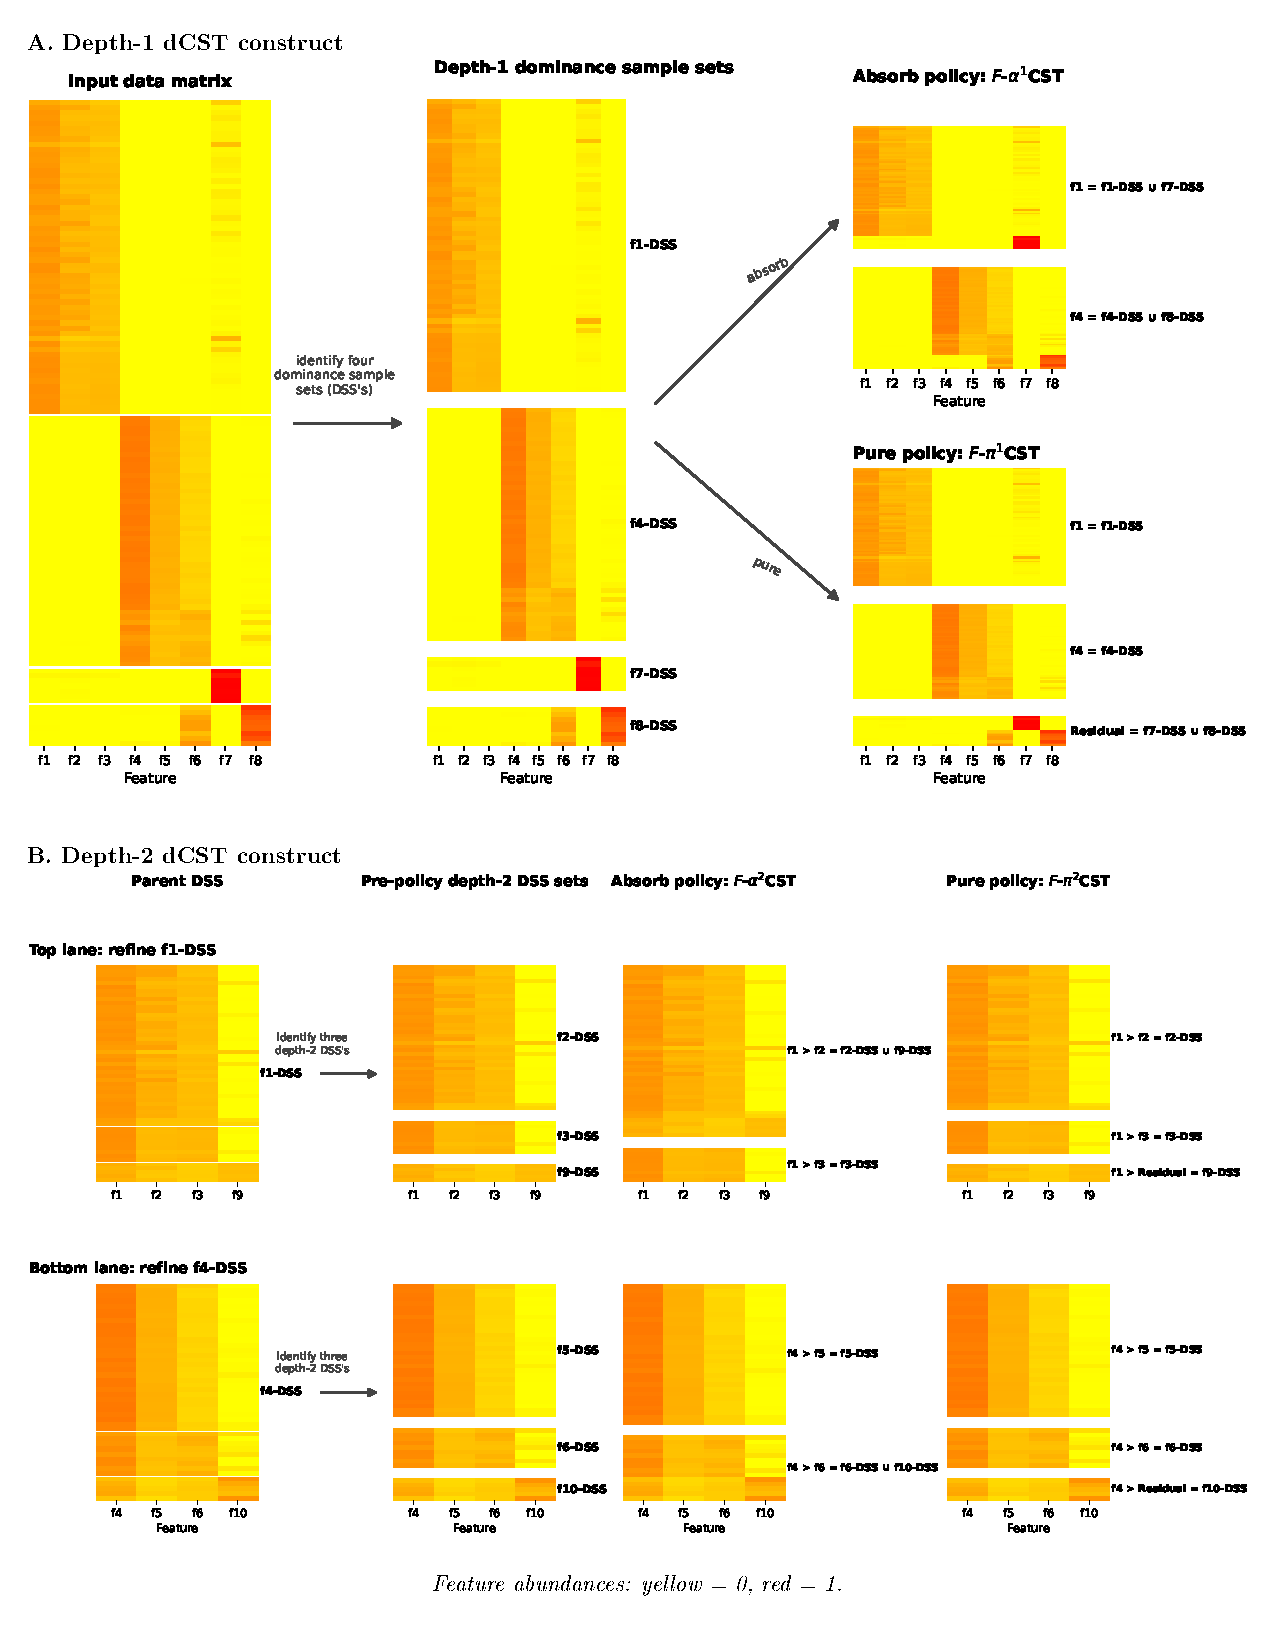
\includegraphics[width=0.98\linewidth,height=0.56\textheight,keepaspectratio]{../assets/figures/FIGURE_1_dcst_conceptual_framework.pdf}
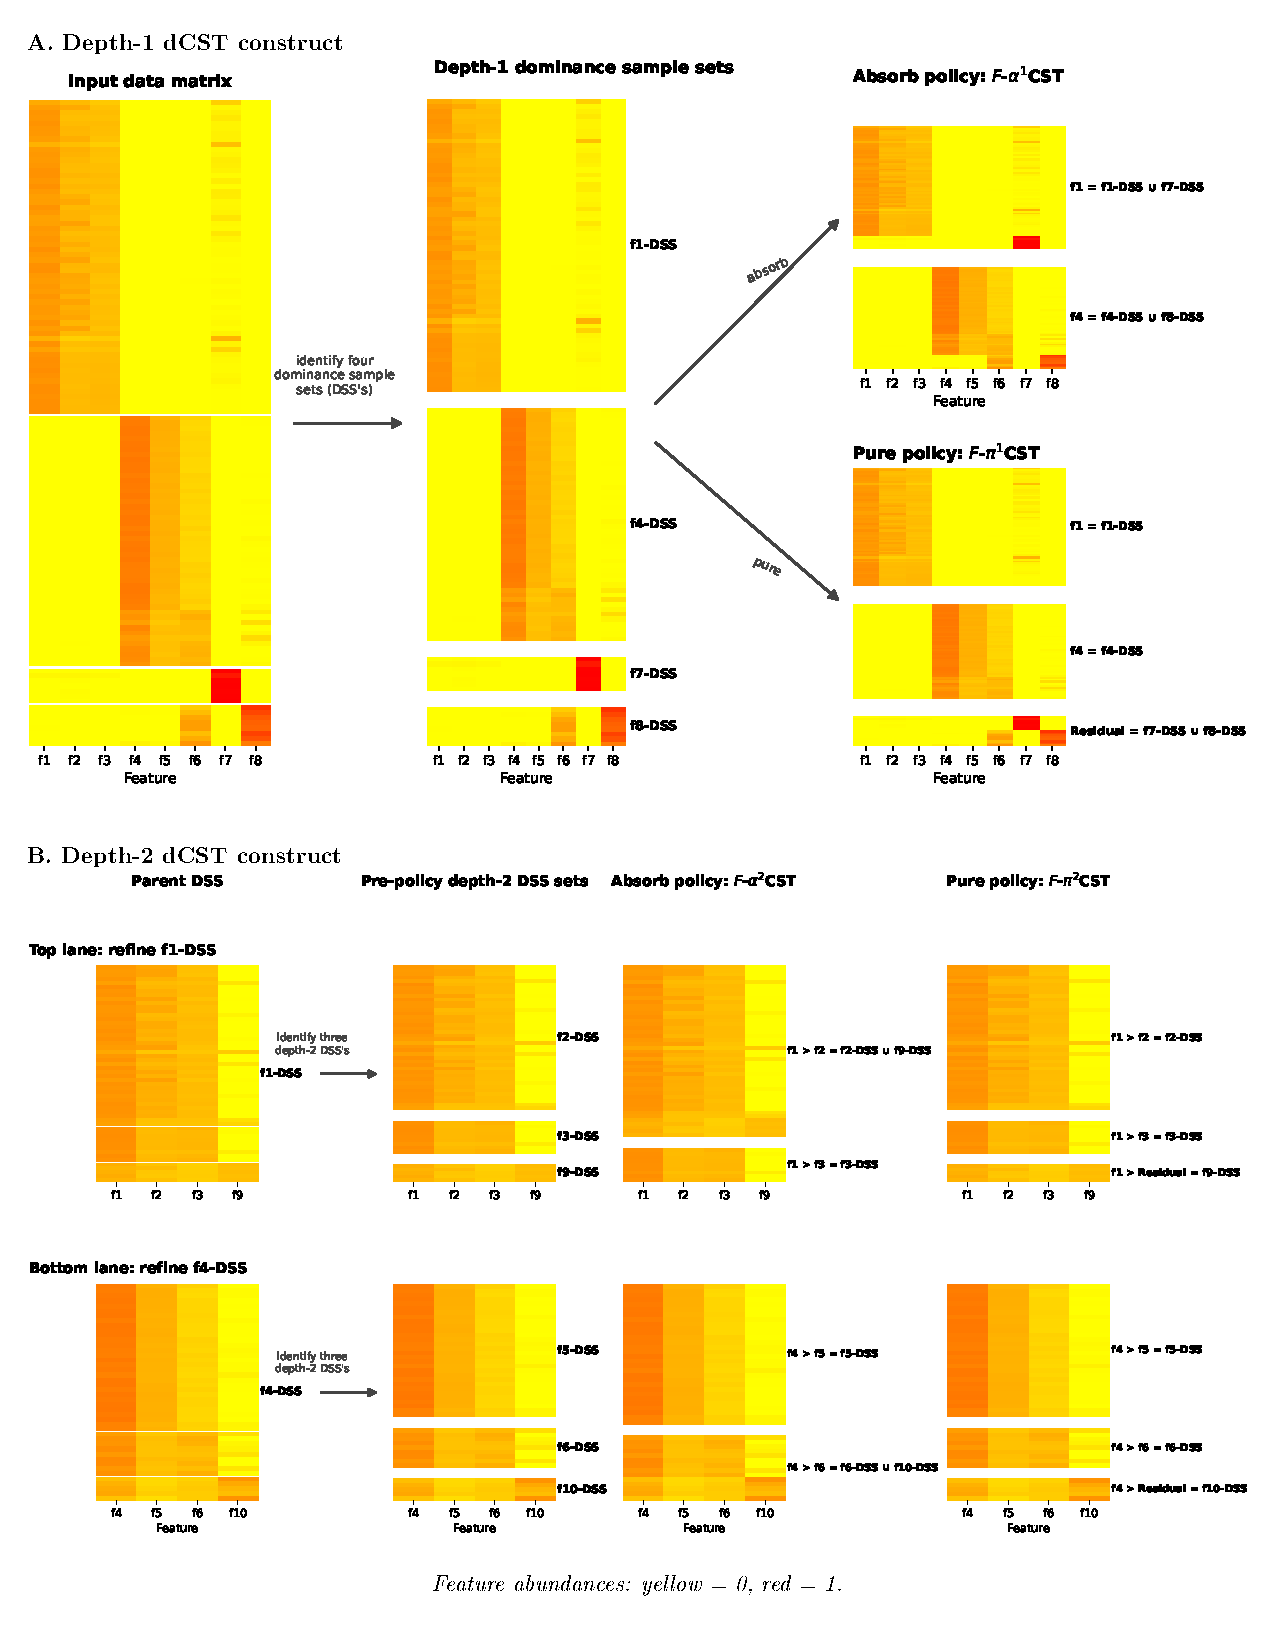
\includegraphics[scale=0.7]{../assets/figures/FIGURE_1_dcst_conceptual_framework.pdf}
\caption{Conceptual dCST construction. Samples are assigned by their dominant
retained feature and recursively refined by the next dominant retained feature
within each retained parent state. The absorb policy reassigns low-support
provisional children into retained sibling states rather than collapsing them
into a residual bucket.}
\label{fig:dcst-concept}
\end{figure}

\FloatBarrier

\section{Methods}

\subsection{dCST framework}\label{sec:dcst-framework}

A dCST hierarchy is a recursive, rank-based partition of a sample-by-feature
abundance matrix whose columns belong to a retained feature family. At depth~1,
each sample is assigned to the state defined by its highest-abundance retained
feature. At depth~2, each retained depth-1 state is refined by the
next-highest-ranked retained feature among the samples that share that parent
assignment, and deeper levels continue the same recursion
(Figure~\ref{fig:dcst-concept}). A depth-$\ell$ dCST
label is therefore a dominance-lineage: an ordered path through a refinement
tree, not a cluster identifier and not a phylogenetic lineage; related
mathematical background is given in \cite{Gajer2025_linf}.

Formally, let \(X \in \mathbb{R}_{\geq 0}^{n \times p}\) be a microbiome
abundance matrix with samples \(i = 1,\ldots,n\) and retained features
\(\mathcal{F} = \{f_1,\ldots,f_p\}\). A depth-1 provisional dominance sample
set for feature \(f\) is
\[
D(f) = \{i : X_{if} = \max_{g \in \mathcal{F}} X_{ig}\},
\]
with ties resolved by the deterministic feature-dictionary-order tie rule, which
selects the first retained feature in the fixed feature-dictionary order when
more than one feature attains the within-sample maximum. Retained
depth-1 states are the dominance sample sets whose support
satisfies the depth-specific minimum \(n_1\), after applying the low-support
policy described below. For
depth \(\ell > 1\), each retained parent lineage
\(L = (f_{a_1},\ldots,f_{a_{\ell-1}})\) with sample set \(S_L\) is refined
within \(S_L\). For each sample in the parent, features already used in the
lineage are ignored and the next highest-abundance retained feature defines a
provisional child. A retained child lineage is therefore
\((f_{a_1},\ldots,f_{a_{\ell-1}}, f_b)\), where \(f_b\) is the next dominant
retained feature among samples in \(S_L\), again subject to the depth-specific
support threshold \(n_\ell\), the same deterministic feature-dictionary-order
tie rule, and the low-support policy. The same recursion defines all fitted
depths.

The absorb policy used in the main analyses handles low-support provisional
children without creating a single residual state. At each parent, provisional
children with support below \(n_\ell\) are reassigned to retained sibling
children within the same parent. For each reassigned sample, the target retained
sibling is the retained child feature with the largest abundance in that sample
among the retained sibling features; ties are resolved by the same deterministic
feature-dictionary-order tie rule applied to the retained-sibling order. Thus
a low-support branch is absorbed into the nearest named dominance context
available at that refinement step. This preserves named dominance-lineages
for downstream comparison while avoiding unstable rare labels.

\newpage
\begin{samepage}
\algorithmtitle{Absorb-policy dCST hierarchy fitting and frozen transfer}
\label{alg:dcst-fit-transfer}
\begin{minipage}{\linewidth}
\small
\textbf{Input:} abundance matrix \(X\); ordered retained feature family
\(\mathcal{F}\); maximum depth \(L_{\max}\); support schedule
\((n_1,\ldots,n_{L_{\max}})\); deterministic tie rule; low-support absorb
policy. Optional transfer input: aligned external matrix \(X^{\ast}\) and a
previously fitted hierarchy.

\textbf{Fit:}
\begin{enumerate}
\item Initialize the root sample set \(S_{\emptyset}=\{1,\ldots,n\}\).
\item For each depth \(\ell=1,\ldots,L_{\max}\), visit every retained parent
lineage \(L\) from depth \(\ell-1\). For each sample \(i\in S_L\), remove from
eligibility the features already present in \(L\), then assign \(i\) to the
eligible retained feature with largest \(X_{if}\); ties are resolved by the
fixed feature-dictionary order. These assignments define provisional child
sets \(P_{L,f}\).
\item Mark provisional children with \(|P_{L,f}|\ge n_\ell\) as retained
children. If no child of \(L\) satisfies this condition, keep \(L\) terminal.
\item For each low-support provisional child \(P_{L,f}\), reassign each
sample \(i\in P_{L,f}\) to the retained sibling \(g\) of the same parent with
largest \(X_{ig}\); ties are resolved by the retained-target order of the
fixed feature dictionary. If no retained sibling has positive abundance in sample \(i\),
use the same ordered fallback retained sibling for that parent.
\item Store the realized lineage sets after absorption and continue recursion
only from retained child lineages.
\end{enumerate}

\textbf{Frozen transfer:}
Align \(X^{\ast}\) to the retained feature dictionary of the fitted hierarchy.
For each external sample and requested nominal depth, follow the same dominance
and tie rules down the frozen realized lineage sets. If the corresponding
reference branch is terminal before the requested nominal depth, assign the
sample to that terminal retained lineage.
\end{minipage}
\end{samepage}

\textit{Determinism and computational cost.} For fixed \(X\), retained feature
order, tie rule, support schedule, and absorb policy, Algorithm~\ref{alg:dcst-fit-transfer}
is deterministic by induction on depth. At depth~1, each sample has a unique
assigned feature because the maximum is evaluated over a fixed ordered feature
set with deterministic tie resolution. If all retained parent sets at
depth~\(\ell-1\) are fixed, then the eligible feature set for every sample in
each parent is fixed, provisional child sets are fixed, support filtering is a
fixed threshold operation, and absorb reassignment uses a fixed ordered maximum
over retained siblings with a deterministic fallback. Thus all retained
depth-\(\ell\) lineage sets are fixed, and the argument continues through all
fitted depths. Frozen transfer is deterministic for the same reason after the
reference hierarchy and feature dictionary have been fixed. A direct dense
implementation has worst-case time \(O(n p L_{\max})\) for fitting or transfer,
excluding feature filtering and downstream inference, with memory dominated by
the input matrix and the stored sample-to-lineage assignments; sparse
implementations reduce the practical scan cost when the retained matrix is
sparse.

\begin{table}[H]
\centering
\footnotesize
\setlength{\tabcolsep}{5pt}
\renewcommand{\arraystretch}{1.15}
\begin{tabularx}{\linewidth}{p{0.23\linewidth}Y}
\toprule
Component & Operational definition \\
\midrule
Input abundance matrix & A non-negative sample-by-feature matrix \(X\). The input may be counts, proportions, or another sample-wise transformation, provided the within-sample order of retained features is preserved; examples include applying the same strictly increasing transformation to all retained feature values within a sample. CLR preserves order for strictly positive compositions, but any zero-replacement or pseudocount step must also preserve within-sample order for the same pre-policy lineage to be guaranteed. \\
Retained feature family & A prespecified feature set \(\mathcal{F}\), such as shared gut taxa or full VOG gene groups, after application-specific filtering. dCST labels are defined only with respect to this retained family. \\
Depth-wise recursion & Depth~1 assigns each sample by its dominant retained feature. Depth~\(\ell\) refines each retained depth-\((\ell-1)\) parent by the next highest retained feature among samples in that parent, excluding features already present in the parent lineage. \\
Low-support absorb policy & Provisional children below the depth-specific support threshold are reassigned to retained sibling states within the same parent, using the largest retained-sibling feature abundance in each reassigned sample. Pure-policy residual states are used only for methodological sensitivity, not for the main analyses. \\
Frozen transfer rule & A hierarchy learned in a reference cohort can be frozen and applied to a new cohort after aligning the new data to the retained feature dictionary. External samples are mapped to realized reference lineage sets at the requested nominal depth; terminal retained lineages remain eligible at later nominal depths when the reference branch did not split further. \\
Rebuilt-cohort mode & As a comparator to frozen transfer, the same feature filtering and absorb-policy workflow can be run independently within an external cohort. Rebuilt mode asks whether related dominance structure is rediscovered without requiring the reference labels themselves to transfer. \\
Panel-level inference & At a fitted depth, the full dCST label-by-outcome table is tested as a panel. We use Fisher-exact contingency-table tests, with Monte Carlo evaluation for large tables, and report Cramer's~V as an omnibus effect-size summary. \\
Label-level inference & Individual dominance-lineages are followed up against all other labels at the same depth using label-versus-rest contrasts, odds ratios, and Benjamini--Hochberg correction within the prespecified family. Bayesian estimates are used as supportive sparse-label summaries. \\
\bottomrule
\end{tabularx}
\caption{Operational dCST construction and inference workflow, summarizing
the formal definition above and the inferential roles used in the main
analyses. Figure~\ref{fig:dcst-concept} gives the intuition;
Algorithm~\ref{alg:dcst-fit-transfer} gives the fitting procedure.}
\label{tab:dcst-workflow}
\end{table}

This construction has three useful properties. First, the pre-policy dominance
lineage of a sample depends only on its within-sample rank order, so the same
pre-policy lineage is recovered from counts, proportions, or any transformation
that preserves the order of retained features within that sample. This includes
the same strictly increasing transformation applied to all retained values in a
sample, such as \(\log(1+x)\) or
arcsine-square-root transformations. For strictly positive compositions, CLR
also preserves within-sample order because it subtracts a sample-specific
constant after the log transform; however, CLR requires zero handling, and a
pseudocount or zero-replacement procedure preserves dCST lineages only if it
preserves within-sample feature order. Transformations that rank-normalize
across samples, residualize features, apply feature-specific scaling, or
otherwise change within-sample order are outside this invariance claim. Second,
the fitted absorb-policy hierarchy is deterministic once the reference cohort,
retained feature family, tie rule, and depth-specific support schedule are
fixed: it does not depend on a clustering algorithm, distance metric,
initialization, or a number-of-clusters parameter. Third, after a hierarchy has
been fitted and frozen, aligned external samples are assigned stably into the
realized lineage sets of that hierarchy. This separates cohort-level hierarchy
fitting from sample-level assignment, in contrast to clustering-defined state
labels whose meaning can drift with the comparison cohort.

Because recursive refinement produces many provisional low-frequency child
states, the hierarchy also requires an explicit low-frequency policy. We use
the absorb policy throughout the primary analyses. Under this policy, provisional
child states below the depth-specific minimum-support threshold are reassigned
into retained named states rather than pooled into a single residual bucket.
This keeps the hierarchy readable and supports direct comparison of named
dominance-lineages across downstream analyses. Pure-policy hierarchies remain
useful as methodological sensitivity analyses, but the analyses here emphasize
absorb-policy dCSTs because they provide a more portable and interpretable
state vocabulary.

\subsection{Shared inferential framework}

The two applications share the same representational core but not a
single rigid downstream statistical template. In both settings we distinguish
panel-level from label-level inference. At a given depth, the primary screen
asks whether outcome labels are distributed non-randomly across the full dCST
panel at that depth. Panel-level tests use Fisher-exact contingency-table tests,
with Monte Carlo evaluation when the full table is large, and summarize panel
strength with Cramer's~V. Label-level follow-up then asks whether individual
dominance-lineages are enriched or depleted relative to the rest of the panel
at the same depth.

Across both applications, multiplicity control is handled with the
Benjamini--Hochberg procedure within the prespecified testing family relevant to
the comparison being reported \cite{BenjaminiHochberg1995}. Odds ratios summarize direction and magnitude at
the label level. Bayesian follow-up is used as a supportive estimation layer,
especially for smaller or deeper states where maximum-likelihood estimates can
be unstable, but it does not replace the frequentist panel-level gate. In both
applications, the dCST representation is fixed first; the downstream tests then
follow the cohort design and available metadata.

Reproducibility settings, including tie handling, Monte Carlo settings,
Bayesian draw counts, and the BH families used in each contrast, are summarized
in Supplementary Table~S3.

Sensitivity to deterministic settings is summarized separately in
Supplementary Table~S4. The tie rule is not treated as a stochastic analysis
choice: it is part of the label definition, and available top-dominance audits
show that exact dominant-feature ties are absent or rare in the matrices
checked. By contrast, the support schedule and retained feature family are
explicit modeling choices. The gut support-schedule audit reports how
\(\pm25\%\) threshold perturbations change pre-policy lineage granularity and
pre-absorb sample coverage, while the CT capped-VOG analyses evaluate robustness
to nested retained-feature caps. These pre-absorb lineage counts are diagnostic
quantities and are distinct from the post-absorb retained-state counts reported
in Table~\ref{tab:fitted-hierarchies}.
These checks do not make dCSTs parameter-free; they make the setting dependence
visible and separate it from clustering algorithm, distance, initialization, and
\(k\) choices.

Downstream analyses differ according to study design. In gut IBD, external
validation and repeated subjects make covariate adjustment and subject-aware
sensitivity essential. In the CT application, label-level enrichment and
Bayesian sparse-state summaries are evaluated inside a fixed outcome-labeled
subset, followed by taxonomic, product, and KEGG-linked interpretation. Thus the
same dCST construction can support application-specific inference without
forcing the two applications into the same statistical design.

\subsection{Gut application design}

The gut application is designed to test portability of taxonomic dCSTs across
cohorts. Structure learning begins with a local American Gut Project stool
table whose amplicon-sequence-variant identifiers were mapped back to sequences
from the corresponding redbiom context and then reassigned taxonomy with the
same DADA2/SILVA workflow used for the external validation datasets. This
shared-taxonomy step places the AGP
discovery cohort and the external validation cohorts in the same label universe
before dCST construction and transfer \cite{McDonald2018_AGP,Quast2013_SILVA}.
We prioritized this shared-feature compatibility over maximizing the number of
AGP samples, because direct transfer is only interpretable when the reference and
validation data are aligned to the same retained-taxon dictionary.

The resulting local AGP source table contained 24,566 samples. Samples with
library size below 1,000 reads were excluded, leaving 24,421
quality-controlled samples after taxon filtering. Retained taxa were required
to reach a count of at least 2 in at least 5\% of the retained samples, which
yielded a 340-taxon discovery matrix. The AGP hierarchy is then
constructed on this filtered AGP matrix under the absorb policy, using a
minimum-support schedule of 50 at depth~1 and 25 at depths~2 through~4. We use
AGP primarily as a large ecological background cohort rather than as a source
of diagnosis-grade IBD case definitions. The AGP phenotype fields are used only
for exploratory prioritization and sensitivity analysis, not as the
primary disease-association evidence.

The primary gut portability evidence comes from external cohorts with stronger diagnosis
metadata. The central comparison separates structure learning from disease
inference: the AGP-derived hierarchy is frozen and external samples are mapped
into it under the corrected nearest-lineage-set transfer rule, while a parallel
rebuilt mode asks whether related dominance structure is rediscovered when each
external cohort is filtered and analyzed independently with the same absorb
workflow. The validation cohorts analyzed here are
Halfvarson 2017, HMP2 / IBDMDB, and Gevers 2014, because they provide the
clearest clinically annotated IBD setting for testing portability. These cohorts
are used to evaluate whether a fitted taxonomic state vocabulary transfers into
compatible disease datasets, not to define a general IBD state classifier. Where
the metadata allow it, the primary contrasts separate pooled IBD, Crohn disease,
and ulcerative colitis \cite{Halfvarson2017_IBD,LloydPrice2019_IBD,Gevers2014_CD}.

Because repeated sampling is a central interpretive issue in the gut data, the
validation layer also includes subject-aware sensitivity analyses. Leading
comparisons are re-evaluated after keeping one sample per subject, and a
bootstrap resample-one-per-subject consensus is used to summarize how strongly
the leading sample-level signals depend on which visit is selected. This
subject-aware layer shows both what transfers and where portability weakens once
longitudinal dependence is taken seriously.

\subsection{CT application design}

The CT application is designed as an independent application of the same
framework in a different niche, feature universe, and biological question. The
labeled CT outcome cohort contains 604 vaginal metagenomic samples (298
spontaneous-clearance and 306 persistence; overall persistence rate 50.7\%).
The clearance/persistence label is the binary endpoint supplied in the parent
CT cohort metadata; detailed enrolment criteria, follow-up duration, and
treatment status for that cohort are documented in the parent CT source, and
the analyses here are association tests against the supplied label rather than
attempts to infer or to recompute the endpoint
\cite{Edwards2019_CTmicrobiota}. These labeled samples are embedded in a
broader 3,602-sample CT+reference cohort consisting of the 604 labeled CT
metagenomes, 434 additional unlabeled CT metagenomes, and 2,564 reference
vaginal metagenomes from the VIRGO2 panel. As in the gut application, the
broader cohort is used for structure learning, while the outcome association
tests remain restricted to the labeled subset.

Unlike the gut application, the CT analysis is gene-family centric. The primary
high-resolution feature universe is a keep-filtered VIRGO2 VOG matrix. Starting
from a combined VOG union table, VOGs are retained only if they are observed in
at least 10 samples and at least 1\% of the combined cohort, yielding the
509,501-VOG universe used for the full-resolution analysis. Smaller 25k, 50k,
100k, and 250k VOG runs are nested robustness analyses drawn from the same
keep-filtered universe by variance ranking \cite{France2026_VIRGO2}. The
full-VOG hierarchy is the primary high-resolution analysis, used to ask whether
CT outcome is distributed non-randomly across deeper gene-family-defined
dominance-lineages and to identify the leading clearance- and
persistence-associated branches. All primary CT hierarchies use the absorb
policy. The capped VOG runs are used as robustness analyses for the full-VOG
result, not as external replication cohorts.

The CT application then adds a biological follow-up layer. Signal-bearing
dominance-lineages are tested for outcome enrichment and interpreted through
consensus taxonomy, representative product annotations, and KEGG-linked
contrasts \cite{Kanehisa2023_KEGG}. This design evaluates whether dCSTs can
organize function-linked metagenomic outcome structure in a biologically
interpretable form, alongside the taxonomic state structure emphasized in the
gut application.

Table~\ref{tab:application-summary} summarizes the two application designs.

\begin{table}[H]
\centering
\footnotesize
\setlength{\tabcolsep}{5pt}
\renewcommand{\arraystretch}{1.18}
\begin{tabularx}{\linewidth}{p{0.16\linewidth} p{0.38\linewidth} Y}
\toprule
Application & Evaluation design & Main interpretation \\
\midrule
Gut (IBD) & Shared-taxonomy stool hierarchy learned in 24,421 local AGP samples, then tested by direct transfer and rebuilt-cohort analysis in external IBD cohorts. & Halfvarson 2017 retained corrected sample-level IBD, Crohn, and UC signal in both transfer and rebuilt modes; subject-aware analyses and HMP2/Gevers boundary cases show that portability is cohort-dependent. \\
CT (vaginal metagenomics) & Full-VOG hierarchy learned in a 3,602-sample CT+reference cohort, with outcome testing restricted to 604 labeled CT samples. & The full-VOG panel reached its strongest CT association at depth~4 ($q = 0.0047$, $V = 0.371$); capped VOG runs supported the panel from 50k features onward, and leading lineages were interpretable through taxonomic, product-level, and KEGG-linked follow-up. \\
\bottomrule
\end{tabularx}
\caption{Complementary application designs. The gut application evaluates
portability and external transfer; the CT application evaluates biological and
functional interpretation in an independent metagenomic setting.}
\label{tab:application-summary}
\end{table}

\subsection{Software}

The dCST construction used here is implemented in the R package
\texttt{linf} version 0.1.0, available under the MIT license at
\url{https://github.com/pgajer/linf}. A tagged release of \texttt{linf} v0.1.0
archived on Zenodo is the canonical reference for this manuscript; the Zenodo
DOI is listed in Data and code availability alongside the corresponding
repository commit. The package provides the operations used here for
sample-wise normalization, dominant-feature assignment, absorb- and pure-policy
dCST construction, recursive refinement, and frozen transfer. The manuscript
analyses combine these package operations with application-specific workflows
for cohort filtering, rebuilt-cohort analysis, association testing, and
biological follow-up. Repository locations, build identifiers, and granular
implementation settings are listed in Data and code availability and
Supplementary Tables~S1--S4.

\section{Results}

A dCST label denotes the within-sample dominance order of retained features at
the relevant depth: in the gut application, depth-2 labels such as
\taxon{Bacteroides~dorei}\dcstsep\taxon{Faecalibacterium~prausnitzii} index a
retained taxonomic dominance-lineage; in the CT application, depth-$\ell$
labels are the analogous gene-family-defined dominance-lineages over the
retained VOG dictionary
(Figure~\ref{fig:dcst-concept}; Table~\ref{tab:application-summary}).

\subsection{Gut application: portability across cohorts}

The gut application begins with a large ecological structure-learning cohort
rather than a diagnosis-grade clinical cohort. In 24,421 quality-controlled AGP
stool samples, the absorb dCST hierarchy contained 50 retained states at
depth~1, 158 at depth~2, 219 at depth~3, and 221 at depth~4. The largest
depth-1 states were centered on \taxon{Bacteroides~dorei},
\taxon{Faecalibacterium~prausnitzii}, and \taxon{Segatella} sp., and the twelve
most common depth-1 states covered 79.8\% of the cohort
(Table~\ref{tab:agp-depth1-landscape}). Exploratory AGP
condition screening identified self-reported IBD as the strongest AGP phenotype
field in this analysis, with Cramer's~V increasing from
0.24 at depth~1 to 0.31 at depth~4. The AGP follow-up itself remained
multistate rather than collapsing to one dominant disease label, with recurrent
enrichment of \taxon{[Eubacterium] eligens group eligens},
\taxon{Alistipes} sp., and deeper \taxon{Bacteroides~dorei}-linked contexts,
together with depletion of \taxon{Segatella} sp. We treat this AGP result as
exploratory prioritization rather than as the main disease evidence because AGP
does not support diagnosis-grade CD/UC subtype interpretation.

\begin{table}[H]
\centering
\caption{Common depth-1 AGP-derived absorb dCST landscape. These twelve
states covered 79.8\% of the 24,421 quality-controlled AGP stool samples
and define the main depth-1 vocabulary used for direct AGP-derived
transfer to external cohorts.}
\label{tab:agp-depth1-landscape}
\footnotesize
\renewcommand{\arraystretch}{1.04}
\begin{tabular}{@{} r l r r r @{}}
\toprule
Rank & dCST & $n$ & Share (\%) & Cumulative (\%) \\
\midrule
1 & \taxon{Bacteroides~dorei} & 8,734 & 35.8 & 35.8 \\
2 & \taxon{Faecalibacterium~prausnitzii} & 3,703 & 15.2 & 50.9 \\
3 & \taxon{Segatella} sp. & 2,557 & 10.5 & 61.4 \\
4 & \taxon{Akkermansia~muciniphila} & 875 & 3.6 & 65.0 \\
5 & \taxon{Agathobacter~faecis} & 846 & 3.5 & 68.4 \\
6 & \taxon{Bacteroides~ovatus} & 578 & 2.4 & 70.8 \\
7 & \taxon{Bacteroides} sp. & 533 & 2.2 & 73.0 \\
8 & Clostridia UCG-014 ord. & 514 & 2.1 & 75.1 \\
9 & \taxon{Bacteroides~fragilis} & 351 & 1.4 & 76.5 \\
10 & \taxon{Bifidobacterium~breve} & 287 & 1.2 & 77.7 \\
11 & UCG-002 sp. & 260 & 1.1 & 78.8 \\
12 & \taxon{Bacteroides~caccae} & 257 & 1.1 & 79.8 \\
\bottomrule
\end{tabular}
\end{table}

The primary gut portability analysis uses external transfer into clinically
richer IBD cohorts. Halfvarson 2017 provided the clearest stool-based support. After
filtering, the pooled branch contained 533 stool samples from 118 subjects, of
which 99 subjects contributed repeated samples. When the frozen AGP-derived
hierarchy was transferred directly into this cohort, pooled IBD, Crohn disease,
and ulcerative colitis all retained corrected sample-level signal. The leading
transferred pattern was biologically coherent across the three
disease-versus-healthy contrasts: depletion of \taxon{Segatella} sp., together
with depletion of \taxon{Akkermansia~muciniphila}, and enrichment of
\taxon{Bacteroides~dorei} in pooled IBD and ulcerative colitis. Rebuilt-cohort
validation in Halfvarson was also positive for pooled IBD, Crohn disease, and
ulcerative colitis, showing that the signal did not depend entirely on exact
AGP label transfer.

Halfvarson also illustrates the limits of sample-level portability. After
one-sample-per-subject sensitivity, the strong sample-level
disease-versus-control transfer contrasts no longer retained $q < 0.05$. Direct
AGP-derived transfer attenuated most strongly, while rebuilt-cohort validation
remained more resilient but still weakened. Rebuilt ulcerative colitis provided
the clearest residual subject-aware pattern, with first-sample
$q = 0.075$, bootstrap recurrence 58.3\%, and median bootstrap odds ratio 5.05,
which we interpret as the strongest remaining subject-aware support rather than
as a second formal BH-significant result. Halfvarson therefore supports
sample-level portability of the representation, but the repeated-sample
structure limits disease-versus-control transfer interpretation.

The most informative within-disease extension in gut was Crohn location, with
ileal-involved versus colonic-only Crohn cases defined according to the
Montreal classification \cite{Satsangi2006_Montreal}.
Relative to colonic-only Crohn disease, ileal-involved Crohn disease was marked
in direct transfer by depletion of \taxon{Faecalibacterium~prausnitzii} and in
rebuilt mode by a stronger depth-2
\taxon{Bacteroides~dorei}\dcstsep\taxon{Faecalibacterium~prausnitzii} contrast
(sample-level odds ratio 0.18, 95\% CI 0.074 to 0.41, $q = 4.4 \times 10^{-5}$).
Under one-sample-per-subject sensitivity, the rebuilt depth-2 contrast remained
the strongest within-disease subject-aware signal in the gut data
($q = 0.042$, bootstrap recurrence 49.6\%, just below the prespecified
50\% working threshold for subject-level stability),
whereas the corresponding AGP-transferred labels attenuated. This asymmetry suggests that
within-disease structure can be present in a rebuilt cohort even
when a frozen external vocabulary does not capture the same subtype boundary
robustly. The rebuilt Crohn-location pattern supports a within-disease
microbiome-state contrast, not only a generic disease-versus-healthy axis, and
its ileal direction is consistent with prior literature on ileal Crohn
disease and adherent-invasive \textit{Escherichia coli}
\cite{DarfeuilleMichaud2004_AIEC_ileal_CD}.

HMP2 / IBDMDB and Gevers 2014 bound the gut portability result.
HMP2 was represented by a mucosal slice rather than stool-equivalent samples and
did not provide broad stool-equivalent replication of the Halfvarson pattern. Gevers
mapped well into the shared-taxonomy hierarchy but
did not retain corrected transferred Crohn-versus-healthy labels in this
pediatric new-onset setting. Exploratory medication follow-up in Gevers did not
restore case-control transfer, suggesting that good mapping into the hierarchy is
not sufficient for portable disease association. Within Gevers Crohn cases,
however, antibiotic exposure was the clearest medication-associated split:
antibiotic-positive samples showed depth-1 transferred \taxon{Bacteroides}
depletion ($q = 0.001$) and depth-2 transferred
\taxon{Escherichia-Shigella}\dcstsep\taxon{Bifidobacterium} enrichment
($q = 0.003$), indicating that the failed Crohn-versus-healthy transfer is
consistent with treatment-shaped community structure dominating the AGP-derived
label space rather than with absence of disease-associated dCST signal in this
cohort. Across these cohorts, the taxonomic dCST vocabulary transferred most
clearly into compatible external IBD data. Transfer strength still depended on
cohort comparability, sample type, and repeated-subject structure. These results
support portable representation under compatible conditions, not broad
validation of an IBD disease-state taxonomy
(Figure~\ref{fig:gut-overview}).

\begin{figure}[!htbp]
\centering
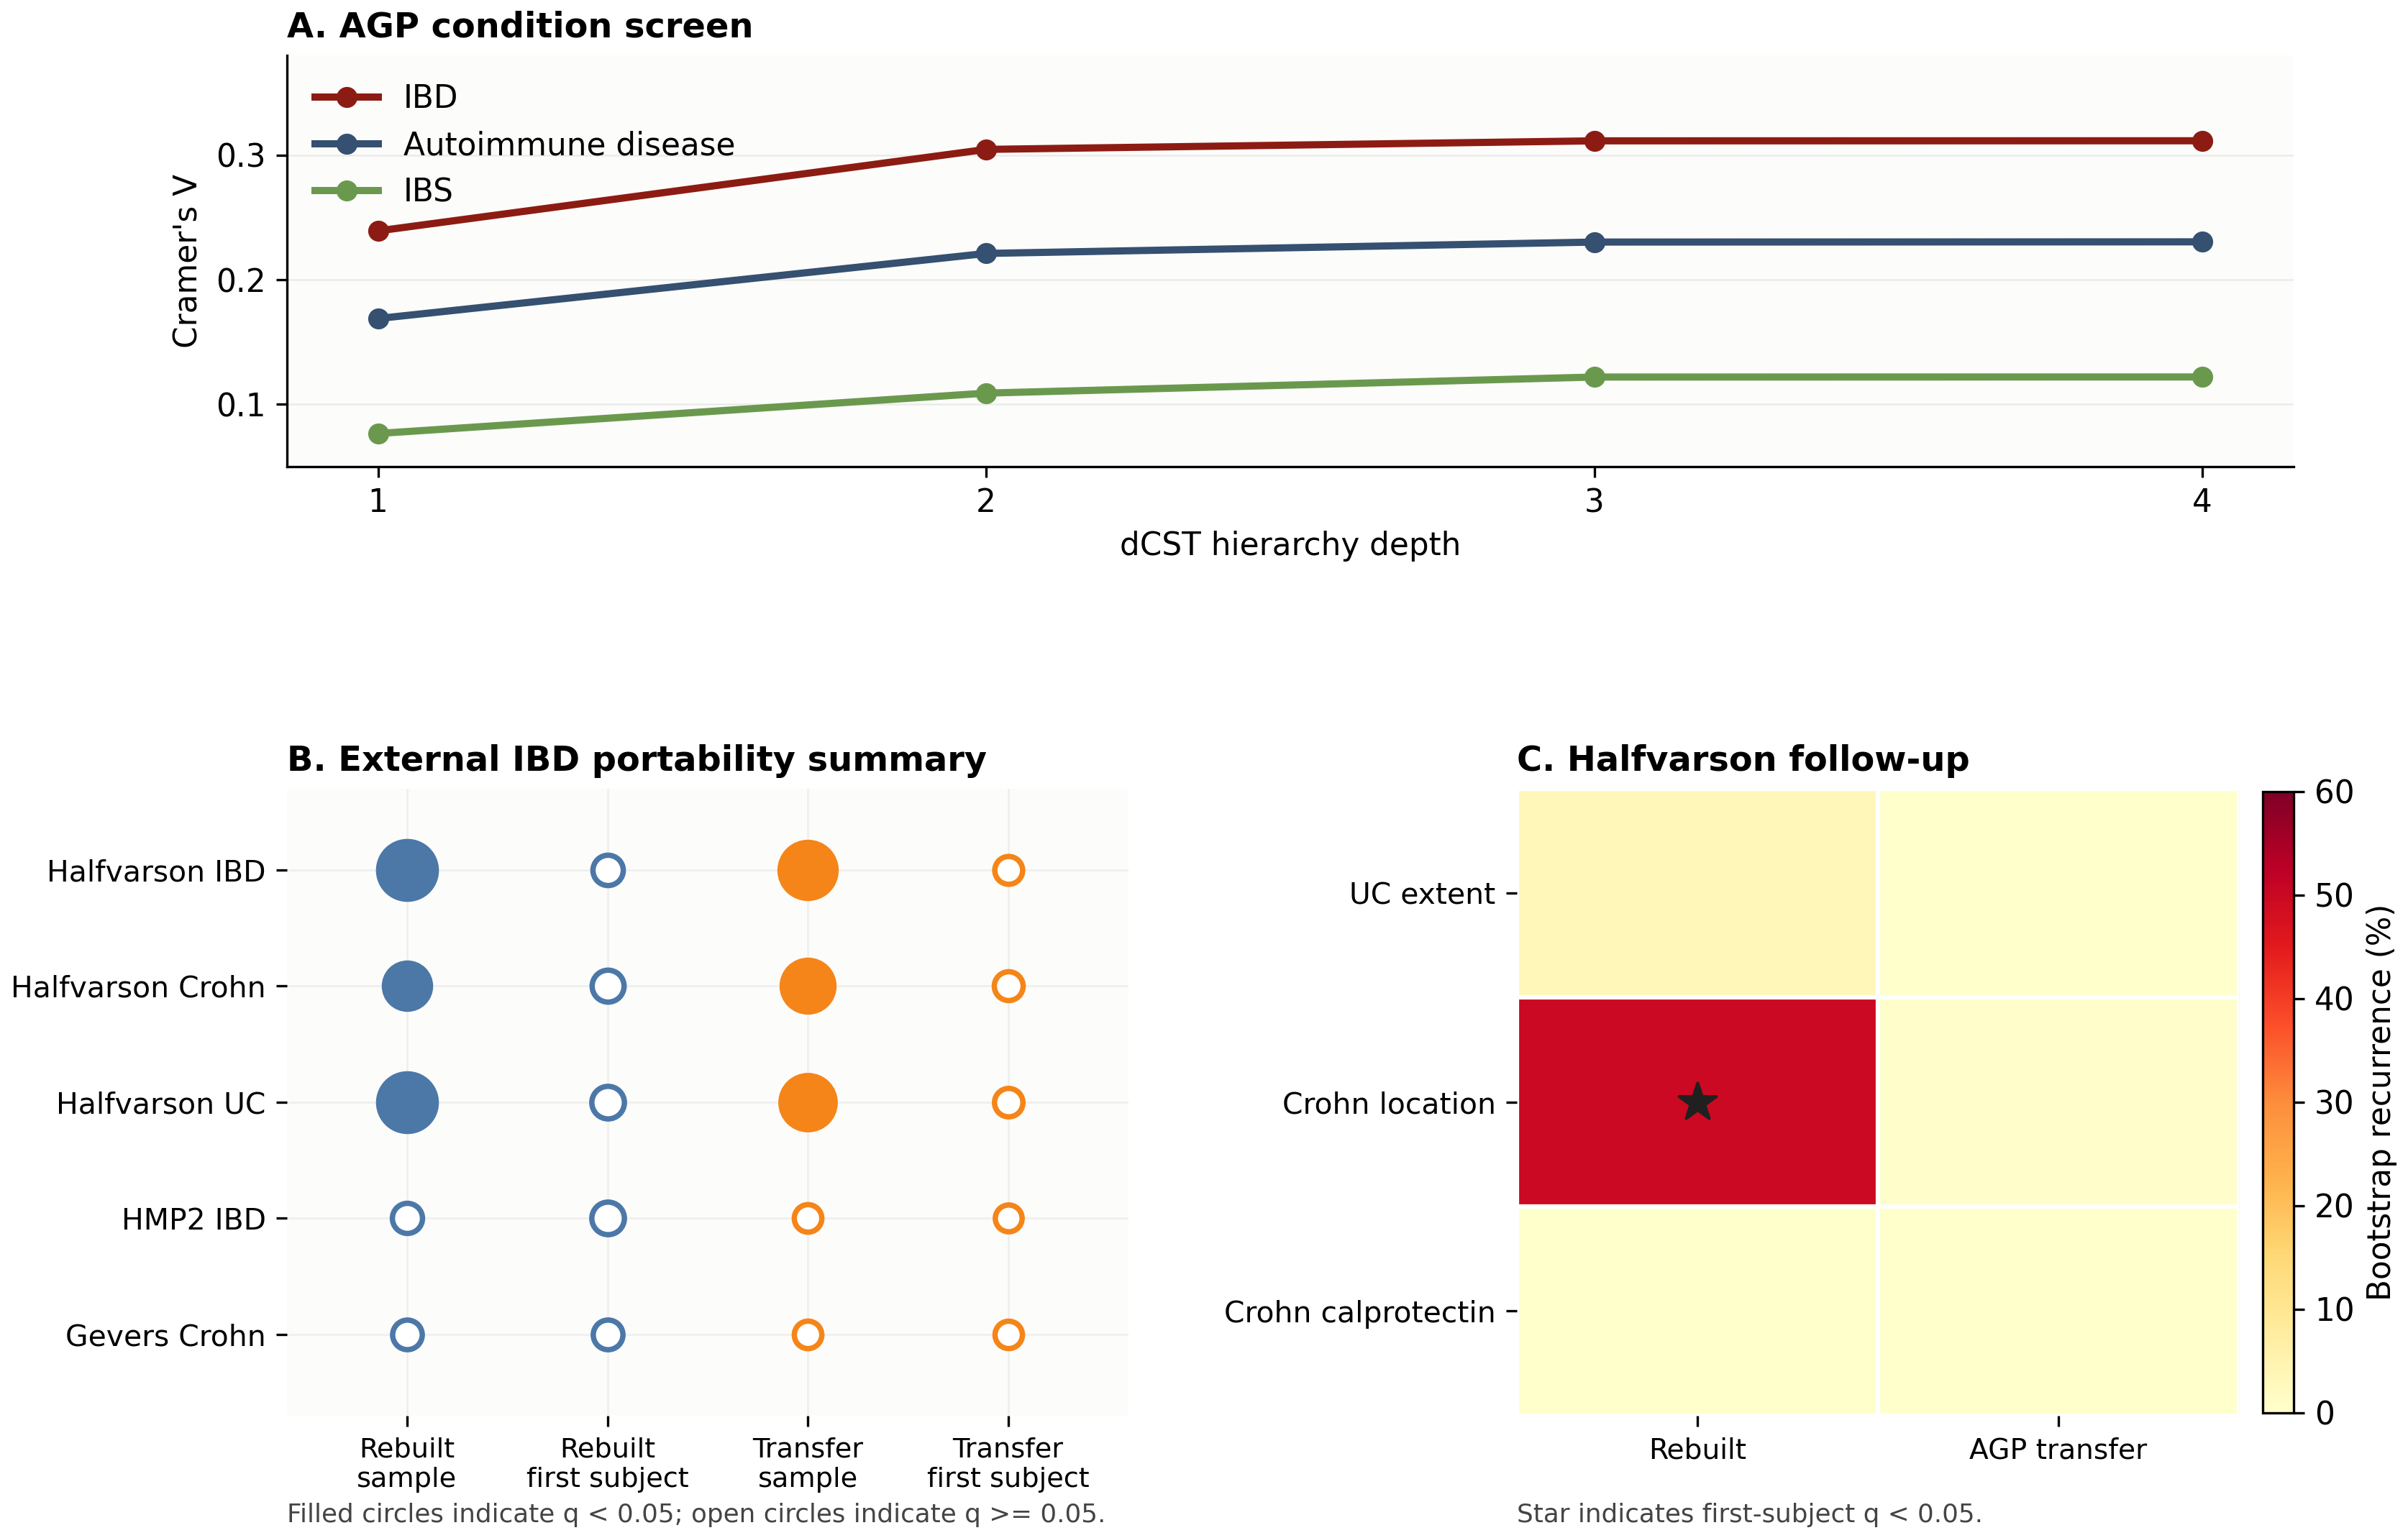
\includegraphics[width=0.96\linewidth,height=0.66\textheight,keepaspectratio]{../assets/figures/FIGURE_2_gut_portability_overview.png}
\caption{Gut portability and subject-aware sensitivity. An AGP-derived
taxonomic dCST vocabulary was evaluated in external IBD cohorts. Panel A shows
the exploratory AGP screen in which self-reported IBD was the strongest AGP
phenotype field retained in the gut analysis. Panel B summarizes external IBD portability without
label-level detail: filled circles indicate corrected \(q < 0.05\), open
circles indicate \(q \geq 0.05\), and marker area scales with corrected signal
strength. Panel C summarizes Halfvarson within-disease follow-up by bootstrap
recurrence; the star marks the rebuilt Crohn-location contrast that retained
first-subject \(q < 0.05\). Halfvarson supports sample-level transfer and
rebuilt-cohort signal, while subject-aware sensitivity and the other external
cohorts bound the portability claim and do not provide broad IBD state
validation.
Expanded label-level details are provided in Supplementary Figure~S1.}
\label{fig:gut-overview}
\end{figure}

\FloatBarrier

\subsection{CT application: outcome-associated and function-linked states}

The CT application addresses a different question from the gut transfer
analysis: whether dCSTs can organize vaginal metagenomic outcome structure in a
biologically interpretable form. The broad
3,602-sample CT+reference cohort provides the ecological background for
learning full-VOG hierarchies, while every outcome test remains restricted to
the same 604 labeled CT metagenomes.

The primary CT result comes from the full 509,501-VOG hierarchy. In this
high-resolution analysis, CT outcome is distributed non-randomly across the
panel at every fitted depth and reaches its strongest panel-level effect at
depth~4 ($q = 0.0047$, Cramer's $V = 0.371$ on the depth-4 CT-occupied panel of
58 dominance-lineages by 2 outcome columns). The signal is distributed across
a gene-family-defined dCST panel rather than concentrated in a single
deterministic VOG biomarker: the leading single labels do not pass label-level
BH correction at the same depth (best
within-depth label-level $q = 0.084$ at depth~3 and $q = 0.102$ at depth~4,
versus panel-level $q = 0.0047$). Within that panel, the most stable lineage
is a clearance-oriented
\taxon{Lactobacillus crispatus}/\taxon{Lactobacillus jensenii} branch that
persists from depth~1 through depth~4. At depth~4, the extension
\texttt{VOG0146820 > VOG0741118 > VOG0741686 > VOG0741595} contains 18 CT
samples, of which 15 are clearance and 3 persistence, with Bayesian odds ratio
0.20 (95\% credible interval 0.05 to 0.57). The strongest full-cap
persistence-oriented single lineage is a pure \taxon{L. iners} branch with
Bayesian odds ratio 3.85 (95\% credible interval 1.38 to 12.78), while a
\taxon{Ca. Lachnocurva vaginae}-centered lineage, which carries the strongest
functional follow-up signal, remains directionally persistence-associated.

The capped VOG analyses support this panel-level interpretation. Relative to
the initial 25k-feature run, broader 50k, 100k, and 250k caps moved depth~4 into
reproducible omnibus support, and the full 509,501-VOG fit retained the strongest
depth~4 panel-level result. At the same time, the exact top-ranked sparse labels
were more cap-sensitive than the overall panel signal. Concretely, the
top-ranked direction-specific depth-3 label changed identity across caps:
a \taxon{Ca. Lachnocurva vaginae}-centered persistence lead at the 25k cap was
displaced by an \taxon{L. iners}-centered persistence lead at the 50k cap and
broader, even as the panel-level signal stabilized. We therefore interpret the
CT result at the panel and dominance-lineage level rather than at the
single-label level. It is a robustness-supported within-cohort signal, not
external replication of a fixed single-label biomarker.

The CT analysis also supports deeper biological interpretation. The stable
clearance branch is functionally enriched for sugar transport, carbohydrate-processing,
lactate-linked, and amino-acid transport features, consistent with a protective
\taxon{Lactobacillus}-centered state. On the persistence-oriented side, the
\taxon{Ca. Lachnocurva vaginae} lineage, which carries the strongest
functional follow-up signal even though its label-level odds ratio is smaller
than that of the \taxon{L. iners} branch, shows transport together with
chemotaxis- and flagellar-related features. The follow-up annotations connect
the outcome-associated states to both taxonomy and function at gene-family
resolution.

The CT-subset comparison is consistent with the broader reference background
stabilizing this signal. It also argues against a simple construction artifact.
When the fixed full-VOG reference hierarchy is
restricted back to the 604 labeled CT samples, the CT subset still occupies
most of the reference labels through depth~4. Specifically, reference-to-CT
label purities are 0.88, 0.86, 0.74, and 0.72 across depths~1--4, while
CT-to-reference purities are 0.48, 0.25, 0.38, and 0.37, indicating that
each broader-cohort label tends to map cleanly to one labeled-CT state,
whereas each CT-only label tends to merge several broader-cohort labels.
By contrast, a hierarchy learned
on the CT subset alone becomes much coarser and loses omnibus support after
depth~2. A broader ecological background therefore appears to sharpen the
learned state vocabulary, but the biological association is still evaluated only
in the outcome-labeled subset. In CT, that vocabulary is structurally stable and
interpretable at the functional level
(Figure~\ref{fig:ct-full-vog}).

The CT analysis also illustrates two features of the construction. Panel-level
inference was more stable than single-label inference at high feature dimension:
the omnibus depth-4 panel-level signal was reproducible from the 50k-feature cap
onward, whereas the identity of the single top-ranked direction-specific label
changed across caps. The absorb policy also kept named dominance-lineages at
depth~4 in a 509,501-feature universe rather than collapsing low-support
refinements into one residual bucket, which allowed the clearance and
persistence-oriented branches to be interpreted through taxonomic,
product-level, and KEGG-linked follow-up.

\begin{figure}[!htbp]
\centering
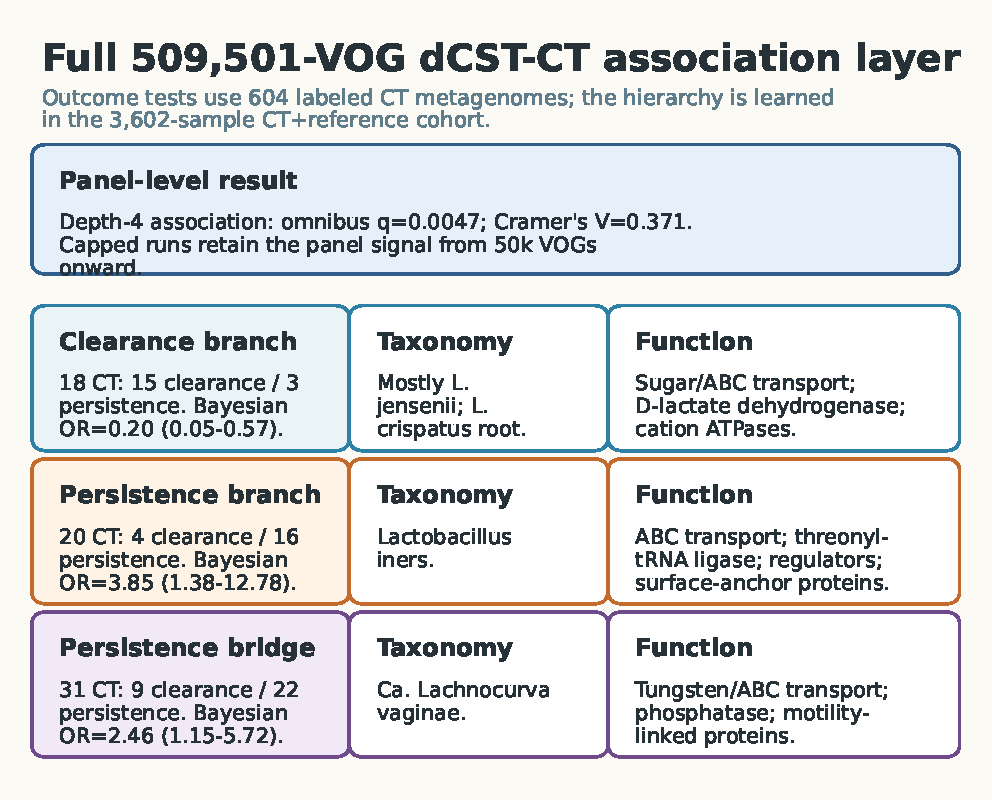
\includegraphics[width=0.95\linewidth,height=0.63\textheight,keepaspectratio]{../assets/figures/FIGURE_3_ct_full_vog_overview.pdf}
\caption{CT full-VOG outcome association and capped-feature robustness.
Clearance- and persistence-associated structure was evaluated across a
high-resolution gene-family dCST panel in the 604 labeled CT metagenomes. The
primary result is a panel-level association in the 509,501-VOG hierarchy, with a
stable clearance-oriented \taxon{Lactobacillus crispatus}/\taxon{Lactobacillus
jensenii} branch and persistence-oriented \taxon{L. iners} and
\taxon{Ca. Lachnocurva vaginae} structure. Capped VOG runs support the
panel-level result from 50k features onward, while single-label rankings are
more cap-sensitive. The CT evidence is a robustness-supported lineage-and-panel
signal, not external replication of one fixed biomarker.
Short branch names are used for readability: the
clearance branch corresponds to
\texttt{VOG0146820 > VOG0741118 > VOG0741686 > VOG0741595}, the
\taxon{L. iners} persistence branch to
\texttt{VOG0418718 > VOG0418741 > VOG0418778}, and the
\taxon{Ca. Lachnocurva} persistence-oriented lineage (smaller label-level OR
than the \taxon{L. iners} branch but the strongest functional follow-up signal)
to \texttt{VOG0675840 > VOG0676581 > VOG0675786}. Visual conventions in this
figure differ from those in Figure~\ref{fig:gut-overview}: the gut overview
encodes corrected significance with filled vs.\ open circles and marker area,
whereas this figure uses named branch labels to identify the leading
clearance- and persistence-oriented lineages.}
\label{fig:ct-full-vog}
\end{figure}

\FloatBarrier

\subsection{Cross-application synthesis}

The two applications probe complementary properties of the same representation:
gut tests portability of a deterministic taxonomic state vocabulary across
external cohorts, while CT tests within-cohort biological interpretation across
a much larger feature universe. In both settings, deeper dCST refinement exposed
additional outcome structure, although the analyses used different tests and
effect-size scales (Figure~\ref{fig:cross-app-synth}). The common point is the
representation itself: deterministic assignment and interpretable
dominance-lineages provide a stable substrate for microbiome state analysis,
while portability, robustness, and biological interpretation remain empirical
properties of each application.

\begin{figure}[!htbp]
\centering
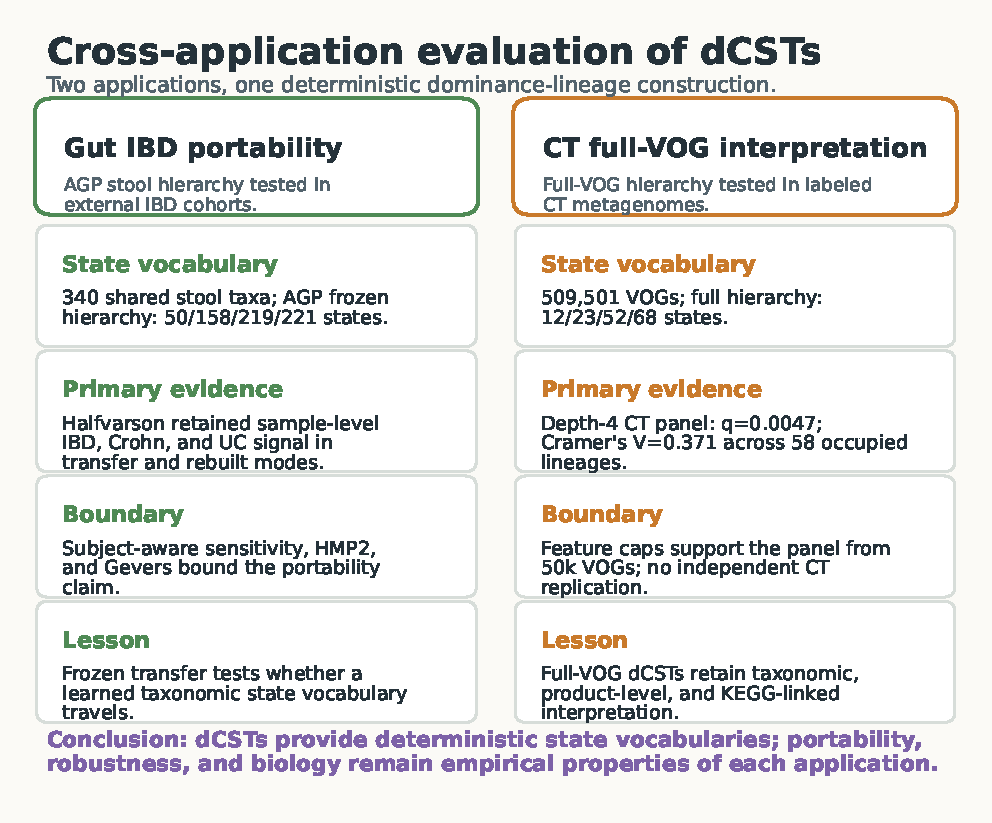
\includegraphics[width=0.95\linewidth,height=0.55\textheight,keepaspectratio]{../assets/figures/FIGURE_4_cross_application_synthesis.pdf}
\caption{Cross-application synthesis. The gut application asks whether an
AGP-derived taxonomic dCST vocabulary transfers into external IBD cohorts and
how that signal changes under subject-aware sensitivity; the CT application
asks whether full-VOG dCSTs organize clearance- and persistence-associated
metagenomic states with taxonomic and functional follow-up. The shared claim is
about the reusable representation, not a universal label set.}
\label{fig:cross-app-synth}
\end{figure}

\FloatBarrier

\section{Discussion}

We asked whether microbiome state labels can be made deterministic and
interpretable without relying on clustering-defined CST or enterotype
constructs. dCSTs replace cluster membership with retained-feature
dominance-lineages: the pre-policy dominance order is defined sample by sample,
the absorb-policy hierarchy is deterministic for a fixed reference cohort and
support schedule, and frozen transfer then assigns aligned samples stably into
the realized lineage sets of that hierarchy. This turns a microbiome state
label from a model-fit cohort-level partition into an object that can be named,
transferred, and interrogated sample by sample.

The comparison to clustering-defined CSTs is definitional, not a claim that a
particular clustering algorithm performs poorly. A clustering-derived label is
conditional on choices such as distance metric, clustering algorithm,
initialization, and number of clusters, whereas an absorb-policy dCST label is
determined by the retained feature family, deterministic tie handling, and the
support schedule. The applications ask whether this deterministic
representation is useful in practice; they do not benchmark one selected
clustering implementation against dCSTs on a particular dataset. Supplementary
Figure~\ref{fig:supp-clustering-contrast} gives a small real-data illustration
using AGP gut example samples: PAM/enterotype-style labels based on
Jensen--Shannon distance change when \(k\) or the comparison set changes,
whereas the same target samples retain identical labels when read through an
already frozen depth-2 dCST assignment.

This distinction matters when comparing dCSTs with existing microbiome state
frameworks. We do not claim that dCSTs replace all of them. PAM-style
enterotypes summarize large gut datasets by clustering samples in a distance space
\cite{Arumugam2011_enterotypes,Costea2018_enterotypes,Knights2014_rethinking};
Dirichlet-multinomial mixture models provide a generative probabilistic
clustering framework for count data \cite{Holmes2012_DMM}; and VALENCIA
provides a nearest-centroid classifier for established vaginal bacterial CSTs
based on 16S rRNA amplicon profiles \cite{France2020_VALENCIA}. A direct
empirical cross-tabulation between dCSTs and VALENCIA-CSTs is out of scope for
this paper: VALENCIA's centroids are trained on 16S amplicon data,
whereas the CT dCST analysis is gene-family-defined on a VIRGO2 metagenomic
matrix, and a head-to-head comparison would require a 16S-equivalent profile of
the same 604 CT samples that does not exist in the present cohort. These
approaches are useful when the scientific goal is cluster discovery,
probabilistic mixture modeling, or assignment to a curated centroid vocabulary
in their respective input modalities. dCSTs address a narrower representation
problem: given a retained feature family and support policy, define a
deterministic rank-based state label that can be frozen, transferred, rebuilt,
and tested without choosing a distance-based clustering partition.

The gut application shows where that strategy worked and where it weakened.
Using a shared-taxonomy AGP reference, the analysis learned a taxonomic dCST
vocabulary that transferred meaningful IBD-associated structure into an
independent stool cohort with stronger diagnosis metadata. The transferred
signals in Halfvarson were sample-level significant and biologically coherent,
and rebuilt-cohort follow-up showed that related dominance structure could be
rediscovered even without freezing the AGP labels. The same results show why
sample-level signal should not be confused with subject-level stability. Once
repeated samples were collapsed or
re-selected at the subject level, the direct disease-versus-control transfer
signal weakened substantially. The gut application supports portable
representation under compatible cohort conditions. It does not provide broad
IBD disease-state validation or a stand-alone diagnostic test.

The CT application tests a different use case. Here, dCSTs remained informative
in a different body site, with a different feature universe, and with a richer
biological follow-up layer. The
full-VOG hierarchy showed that CT outcome is organized across a
high-resolution gene-family-defined panel. The larger capped VOG runs showed
that the panel-level signal stabilizes from 50k features onward, supporting the
CT result as a within-cohort robustness finding rather than external
replication. The clearance-oriented
\taxon{Lactobacillus crispatus}/\taxon{Lactobacillus
jensenii} branch, the persistence-oriented \taxon{L. iners} and
\taxon{Ca. Lachnocurva vaginae} structure, and the supporting transport,
lactate, flagellar, and chemotaxis annotations together show that dCSTs can
anchor biological interpretation rather than merely partition samples.

The two analyses support different claims. The gut
analysis addresses external transfer and rebuilt-cohort behavior in clinically
annotated IBD datasets, with explicit limits imposed by cohort mismatch and
repeated-subject structure. The CT analysis addresses within-cohort
gene-family-level outcome interpretation and feature-cap robustness, but does
not provide an external CT replication cohort. Across both, dCSTs separate
state construction from downstream inference: the same kind of fitted
vocabulary can be used for transfer and rebuilt comparisons in gut, and for
outcome association with functional follow-up in CT, without claiming a
universal state vocabulary, a diagnostic classifier, a causal mechanism, or
guaranteed portability in every microbiome setting.

Several limitations remain important. First, deterministic labels do not
guarantee strong biological signal. A dCST vocabulary can be cleanly defined
and still prove only modestly portable in some cohorts. Second, shared feature
universes matter. The gut results improved materially once the AGP discovery
cohort and the external validation cohorts were placed in a common taxonomy
universe, and the CT application likewise depended on a clearly defined VOG
feature family. Third, deterministic construction should not be confused with
robustness to every possible setting: support schedules and retained-feature
filters control the granularity of the fitted hierarchy and should be reported
as part of the analysis definition. Fourth, the framework is descriptive rather
than causal. A
dominance-lineage associated with persistence, clearance, or disease does not
by itself explain mechanism. Even in the CT application, where the follow-up
layer is richer, the taxonomic, product, and KEGG results should be read as
biological interpretation and hypothesis generation rather than as resolved
mechanistic evidence.

The next steps are straightforward. In gut, subject-aware inference should be
strengthened in cohorts with more unique controls, richer subtype metadata, and
additional molecular layers. In CT, independent vaginal metagenomic cohorts are
needed to test external replication of the leading VOG-defined states, and
targeted mechanistic work is needed to evaluate the transport- and
motility-linked annotations. More broadly, dCSTs are most useful as a stable
interface between high-dimensional microbiome measurements and downstream
biological interpretation, particularly when taxonomic, functional, and clinical
data are analyzed together. Potential applications include cross-cohort
meta-analysis standardization, pre-specified trial stratification, and
longitudinal monitoring; each requires prospective validation before clinical
use.

\section{Data and code availability}

The manuscript source and figure assets are maintained in the
\texttt{linf} repository: \url{https://github.com/pgajer/linf}. This build was
compiled from the local \texttt{linf} working tree based on commit
\texttt{d89c3de5281d610328dc802a210c6b5d410e5454} at \manuscriptbuilddatetime.
The tagged \texttt{linf} v0.1.0 release used for the analyses in this
manuscript is archived on Zenodo (DOI to be inserted at acceptance) and
is the canonical citation for the package. Gut
application discovery, transfer, rebuilt-cohort validation, and sensitivity
analyses are maintained in the \texttt{gut\_microbiome}
repository: \url{https://github.com/pgajer/gut_microbiome}; the current build
uses local analyses based on commit
\texttt{811cafc07dba9a3fef5a843ef1a25e9fc4de0d70}, with a tagged release
archived on Zenodo (DOI to be inserted at acceptance). CT application
analyses are maintained in the \texttt{CT\_clearance} repository:
\url{https://github.com/pgajer/CT_clearance}; the current CT assets are based on
commit \texttt{de9c7444b07251bfc64e28c2cc15771d1dec6c0e}, also tagged and
archived on Zenodo (DOI to be inserted at acceptance). For final submission,
the Zenodo DOIs are the canonical archival references; the commit hashes are
included for short-term traceability of the build. Implementation
details are summarized in the supplement.
Minimal reproduction requires rerunning the gut analysis workflow in
\texttt{gut\_microbiome}, the CT analysis workflow in
\texttt{CT\_clearance}, and the manuscript build workflow in \texttt{linf}.

The supplement also maps the conceptual dCST operations in
Algorithm~\ref{alg:dcst-fit-transfer} to the corresponding \texttt{linf}
package functions. The gut application uses the local American Gut Project
shared-taxonomy stool
table derived from \texttt{PRJEB11419} together with the external IBD cohorts
summarized in Supplementary Table~S1. The CT application uses
the 604-sample outcome-labeled CT cohort embedded in the 3,602-sample
CT+reference cohort summarized in Supplementary Table~S1. Supplementary
Tables~S1--S4 summarize the cohort counts, feature families, filtering
thresholds, support schedules, tie handling, Monte Carlo and Bayesian settings,
multiple-testing families, transfer rules, and implementation details for the
analyses reported here.

\section{Funding}

\paperfundingnote

\section{Competing Interests}

The authors declare no competing interests.

\section{Acknowledgments}

We thank the participants and investigators of the American Gut Project,
Halfvarson 2017, HMP2 / IBDMDB, PRJEB84421, and Gevers 2014 for making the gut
cohort resources available. We also thank the investigators and participants
behind the CT outcome-labeled and vaginal reference resources used in the
vaginal metagenomic application, and we thank the VIRGO2 project context that
made the gene-family-based CT analysis possible.

\bibliographystyle{unsrt}
\bibliography{combined_references}

\clearpage
\appendix
\FloatBarrier
\begin{landscape}
\begingroup
\scriptsize
\setlength{\tabcolsep}{4pt}
\renewcommand{\arraystretch}{1.16}

\section*{Supplementary Information}

\noindent\textbf{Supplementary Table S1.} Cohorts, sample counts, and feature
families used in the dCST applications.

\begin{longtable}{p{0.16\linewidth}p{0.38\linewidth}p{0.38\linewidth}}
\toprule
Analysis layer & Cohorts and sample counts & Feature family and filtering \\
\midrule
\endfirsthead
\toprule
Analysis layer & Cohorts and sample counts & Feature family and filtering \\
\midrule
\endhead
\bottomrule
\endfoot
Gut AGP discovery and exploratory prioritization &
Local AGP stool table derived from PRJEB11419; 24,566 source samples and 24,421 quality-controlled samples after library-size and all-zero post-filter exclusions. AGP phenotype fields were used for exploratory prioritization, not diagnosis-grade CD/UC inference. &
Shared-taxonomy stool taxon matrix. ASV sequences were reassigned with the DADA2/SILVA workflow used for the external cohorts. Retained taxa required count \(\geq 2\) in at least 5\% of retained samples, yielding 340 taxa. \\
\midrule
Gut external IBD transfer and rebuilt-cohort analysis &
Main external IBD cohorts: Halfvarson 2017 stool branch, 533 samples from 118 subjects for pooled IBD versus healthy; HMP2/IBDMDB mucosal slice, 166 samples from 81 subjects; Gevers 2014 Crohn-focused stool branch, 396 samples from 363 subjects. Halfvarson subtype branches contained 200 Crohn-case samples from 49 subjects and 279 UC-case samples from 60 subjects, each compared with 54 healthy-control samples from 9 subjects. &
External cohorts were aligned to the AGP retained-feature dictionary for direct transfer. Rebuilt analyses used cohort-specific filtered matrices under the same absorb workflow, allowing related dominance structure to be rediscovered without requiring exact AGP labels. \\
\midrule
CT full-VOG hierarchy, capped robustness runs, and functional follow-up &
The 3,602-sample CT+reference learning cohort contained 604 outcome-labeled CT metagenomes, 434 additional unlabeled CT metagenomes, and 2,564 VIRGO2 reference metagenomes. The 604 labeled CT samples were used for all CT outcome contrasts: 298 spontaneous-clearance and 306 persistence samples. &
Primary high-resolution feature family was the keep-filtered VIRGO2 VOG matrix. From 960,439 VOGs in the combined union table, VOGs were retained if observed in at least 10 samples and at least 1\% of the combined cohort, yielding 509,501 VOGs. Capped robustness runs used 25k, 50k, 100k, and 250k VOG subsets drawn from the same retained universe by variance ranking. \\
\midrule
Cross-application synthesis and assets &
The synthesis integrates the gut transfer/rebuilt analyses and CT full-VOG analyses as complementary evaluations of the dCST state vocabulary. &
No new feature family is introduced for the synthesis; it reuses the gut shared-taxonomy and CT full-VOG feature families above. \\
\end{longtable}

\clearpage

\noindent\textbf{Supplementary Table S2.} dCST construction, testing families,
and transfer rules used in the dCST applications.

\begin{longtable}{p{0.16\linewidth}p{0.34\linewidth}p{0.42\linewidth}}
\toprule
Analysis layer & dCST support schedule & Testing, BH family, and transfer rule \\
\midrule
\endfirsthead
\toprule
Analysis layer & dCST support schedule & Testing, BH family, and transfer rule \\
\midrule
\endhead
\bottomrule
\endfoot
Gut AGP discovery and exploratory prioritization &
Absorb-policy hierarchy fit through depth 4. Minimum support: \(n_0=50\) at depth 1; \(n_0=25\) at depths 2--4. Pure-policy results were retained as sensitivity analyses. &
AGP condition screens and label follow-up used depth-specific panel and label families with Benjamini--Hochberg correction. Bayesian follow-up was supportive; BH-adjusted frequentist results were treated as screen-level evidence. No external transfer is involved in this discovery row. \\
\midrule
Gut external IBD transfer and rebuilt-cohort analysis &
Direct transfer used the frozen AGP absorb hierarchy through depths 1--4. Rebuilt-cohort analyses used the same absorb-policy construction and depth range used for the AGP-derived hierarchy. &
Direct transfer used \texttt{transfer.dcsts()} with the corrected nearest-lineage-set rule: external samples were compared against realized AGP lineage sets at each nominal depth, and stable terminal lineages remained assignable at later nominal depths. Rebuilt mode analyzed each external cohort independently. Label-level and panel-level tests used BH correction within the prespecified comparison/mode/depth families. Repeated-subject sensitivity retained one sample per subject and used bootstrap one-sample-per-subject recurrence for leading rows. \\
\midrule
CT full-VOG hierarchy, capped robustness runs, and functional follow-up &
Absorb-policy full-VOG and capped-VOG hierarchies fit through depth 4. Minimum support: \(n_0=50\) at depth 1; \(n_0=25\) at depth 2; \(n_0=12\) at depth 3; \(n_0=10\) at depth 4. &
Primary readout was panel-level CT outcome association across the full dCST label panel at each depth, with BH correction over the prespecified depth-level family. Label-level Fisher tests and Jeffreys-prior Bayesian prevalence contrasts were supportive sparse-label summaries. Product, taxonomy, and KEGG contrasts were descriptive post hoc interpretation layers, not independent discovery gates. No independent CT replication cohort is included. \\
\midrule
Cross-application synthesis and assets &
No additional dCST hierarchy is fit for the synthesis figure. &
The synthesis is descriptive and does not introduce a new testing family. It summarizes the complementary application evidence: gut portability and external transfer, and CT biological and functional interpretability. \\
\end{longtable}

\clearpage

\noindent\textbf{Supplementary Table S3.} Implementation-level settings for
deterministic assignment, stochastic inferential summaries, and multiple-testing
families.

\begin{longtable}{p{0.24\linewidth}p{0.68\linewidth}}
\toprule
Implementation item & Setting used in the reported analyses \\
\midrule
\endfirsthead
\toprule
Implementation item & Setting used in the reported analyses \\
\midrule
\endhead
\bottomrule
\endfoot
dCST package-operation mapping &
The \texttt{linf} package functions used for Algorithm~\ref{alg:dcst-fit-transfer} were: \texttt{normalize.linf()} for sample-wise normalization; \texttt{linf.cells()} for dominant-feature assignment; \texttt{linf.csts()} for depth-1 dCST construction with pure or absorb low-support policies; \texttt{refine.linf.csts()} and \texttt{refine.linf.csts.iter()} for recursive depth-wise refinement, including absorb reassignment; and \texttt{transfer.dcsts()} for assigning aligned samples into a frozen fitted hierarchy. Application-specific repository workflows then performed cohort filtering, rebuilt-cohort analysis, association testing, and biological follow-up. \\
\midrule
dCST tie handling and feature identity &
All primary dCST pipelines used the \texttt{linf} default \texttt{tie.method = "first"}. For primary dominance assignment, tied features are resolved by the fixed feature-dictionary/column order; duplicate feature IDs or labels are made unique before assignment. Absorb reassignment uses the same ordered retained-feature dictionary restricted to the retained sibling targets for the active parent. If a low-support or all-zero sample has no positive retained-sibling value, it is assigned to the fallback retained sibling defined by that same ordered retained-target list. Observed top-feature ties were absent or rare in the reported audits, so tie handling is specified for reproducibility rather than because ties drive the analyses. \\
\midrule
Monte Carlo Fisher settings &
AGP exploratory condition-depth screening used the recorded seed \(20260411\), standard Monte Carlo Fisher mode, and \(B=1{,}000\) simulations per panel in the run reported here. CT full-VOG omnibus panels used Fisher tests with Monte Carlo evaluation and \(B=50{,}000\) simulations per panel. The CT association scripts did not set a separate Fisher-test seed, so exact simulated \(p\)-value digits are reproduced from the generated result tables rather than regenerated deterministically from the script alone. dCST labels themselves do not depend on Monte Carlo draws. \\
\midrule
Bayesian sparse-label summaries &
Gut follow-up used 4,000 posterior draws for Jeffreys-prior beta-binomial prevalence contrasts, \(p_{\mathrm{in}}\sim\mathrm{Beta}(a+0.5,b+0.5)\) and \(p_{\mathrm{out}}\sim\mathrm{Beta}(c+0.5,d+0.5)\), and used \texttt{arm::bayesglm} binomial logistic models for adjusted label-presence summaries when complete-case support was sufficient. Available AGP covariates were host age bin, sex, and BMI. CT follow-up used the same Jeffreys-prior prevalence contrast with 4,000 draws and did not run gut-style adjusted Bayesian logistic regression. CT Bayesian follow-up runs used seeds \(20260411\) and \(20260415\). \\
\midrule
Benjamini--Hochberg families &
AGP exploratory phenotype screening adjusted the eligible phenotype-by-depth omnibus panels as one screen family; AGP label follow-up reported both global label-level BH values across tested labels/depths within each outcome and depth-specific BH values. Gut external transfer and rebuilt-cohort analyses adjusted label tests within each prespecified cohort/comparison/mode/depth family. CT full-VOG and capped-VOG omnibus tests adjusted across depths within each feature-cap run; label-level tests adjusted within each depth panel. \\
\end{longtable}

\clearpage

\noindent\textbf{Supplementary Table S4.} Setting-dependence and robustness
checks for deterministic dCST construction.

\begin{longtable}{p{0.18\linewidth}p{0.48\linewidth}p{0.26\linewidth}}
\toprule
Check & Summary & Interpretation \\
\midrule
\endfirsthead
\toprule
Check & Summary & Interpretation \\
\midrule
\endhead
\bottomrule
\endfoot
Deterministic tie rule & All reported dCST fits used \texttt{tie.method = "first"}: first retained feature for primary dominance and first retained target for absorb reassignment. This is part of the label definition, not a random analysis option. & The reported labels are reproducible by definition once feature order is fixed. \\
\midrule
Observed top-feature ties & Dominant-feature ties were absent in the bundled AGP gut example (0/766 rows) and rare in the CT cap audit: 1/3602 rows in the 50k-VOG cap audit (0.03\%); maximum tied top set size 2. & Tie handling is specified for exact reproducibility; available audits do not suggest that top-feature ties drive the reported examples. \\
\midrule
Gut support-schedule perturbation & Using the existing AGP raw-lineage size audit, a \(\pm25\%\) perturbation around the manuscript support schedule 50/25/25/25 changed pre-policy hierarchy granularity but preserved high pre-absorb sample coverage at shallow depths. These diagnostic counts are pre-absorb raw-lineage counts and should not be compared directly with the post-absorb retained-state counts in Table~1. -25\%: thresholds 38/19/19/19; retained raw lineages 45/170/221/123; pre-absorb retained sample share 96.8\%/83.3\%/52.1\%/16.8\%. nominal: thresholds 50/25/25/25; retained raw lineages 40/141/154/89; pre-absorb retained sample share 96.2\%/81.3\%/47.4\%/14.4\%. +25\%: thresholds 63/31/31/31; retained raw lineages 35/115/114/64; pre-absorb retained sample share 95.3\%/79.0\%/43.8\%/12.1\%. & The support schedule controls naming granularity and should be treated as an explicit modeling choice, not as a hidden clustering parameter. \\
\midrule
CT retained-feature cap robustness & Capped VOG analyses used nested variance-ranked subsets from the same 509,501-VOG retained universe. 25k: depth-3 q=0.0414, V=0.325, depth-4 q=0.2125; 50k: depth-3 q=0.0053, V=0.360, depth-4 q=0.0074; 100k: depth-3 q=0.0042, V=0.358, depth-4 q=0.0063; 250k: depth-3 q=0.0044, V=0.357, depth-4 q=0.0053; 509,501: depth-3 q=0.0046, V=0.357, depth-4 q=0.0047. The 25k cap was shallower, whereas 50k and larger caps retained depth-4 support. & This supports the CT result as a within-cohort feature-family robustness result, not as external replication. \\
\midrule
Gut feature-filter scope & The gut taxonomic analysis is conditional on the stated shared-taxonomy retained family: count \(\geq2\) in at least 5\% of retained AGP samples, yielding 340 taxa. The combined manuscript does not claim robustness to all alternative gut prevalence filters. & This bounds the gut portability claim to the retained feature family used for transfer and rebuilt analyses. \\
\end{longtable}


\endgroup
\end{landscape}


\FloatBarrier
\setcounter{figure}{0}
\renewcommand{\thefigure}{S\arabic{figure}}

\begin{figure}[!p]
\centering
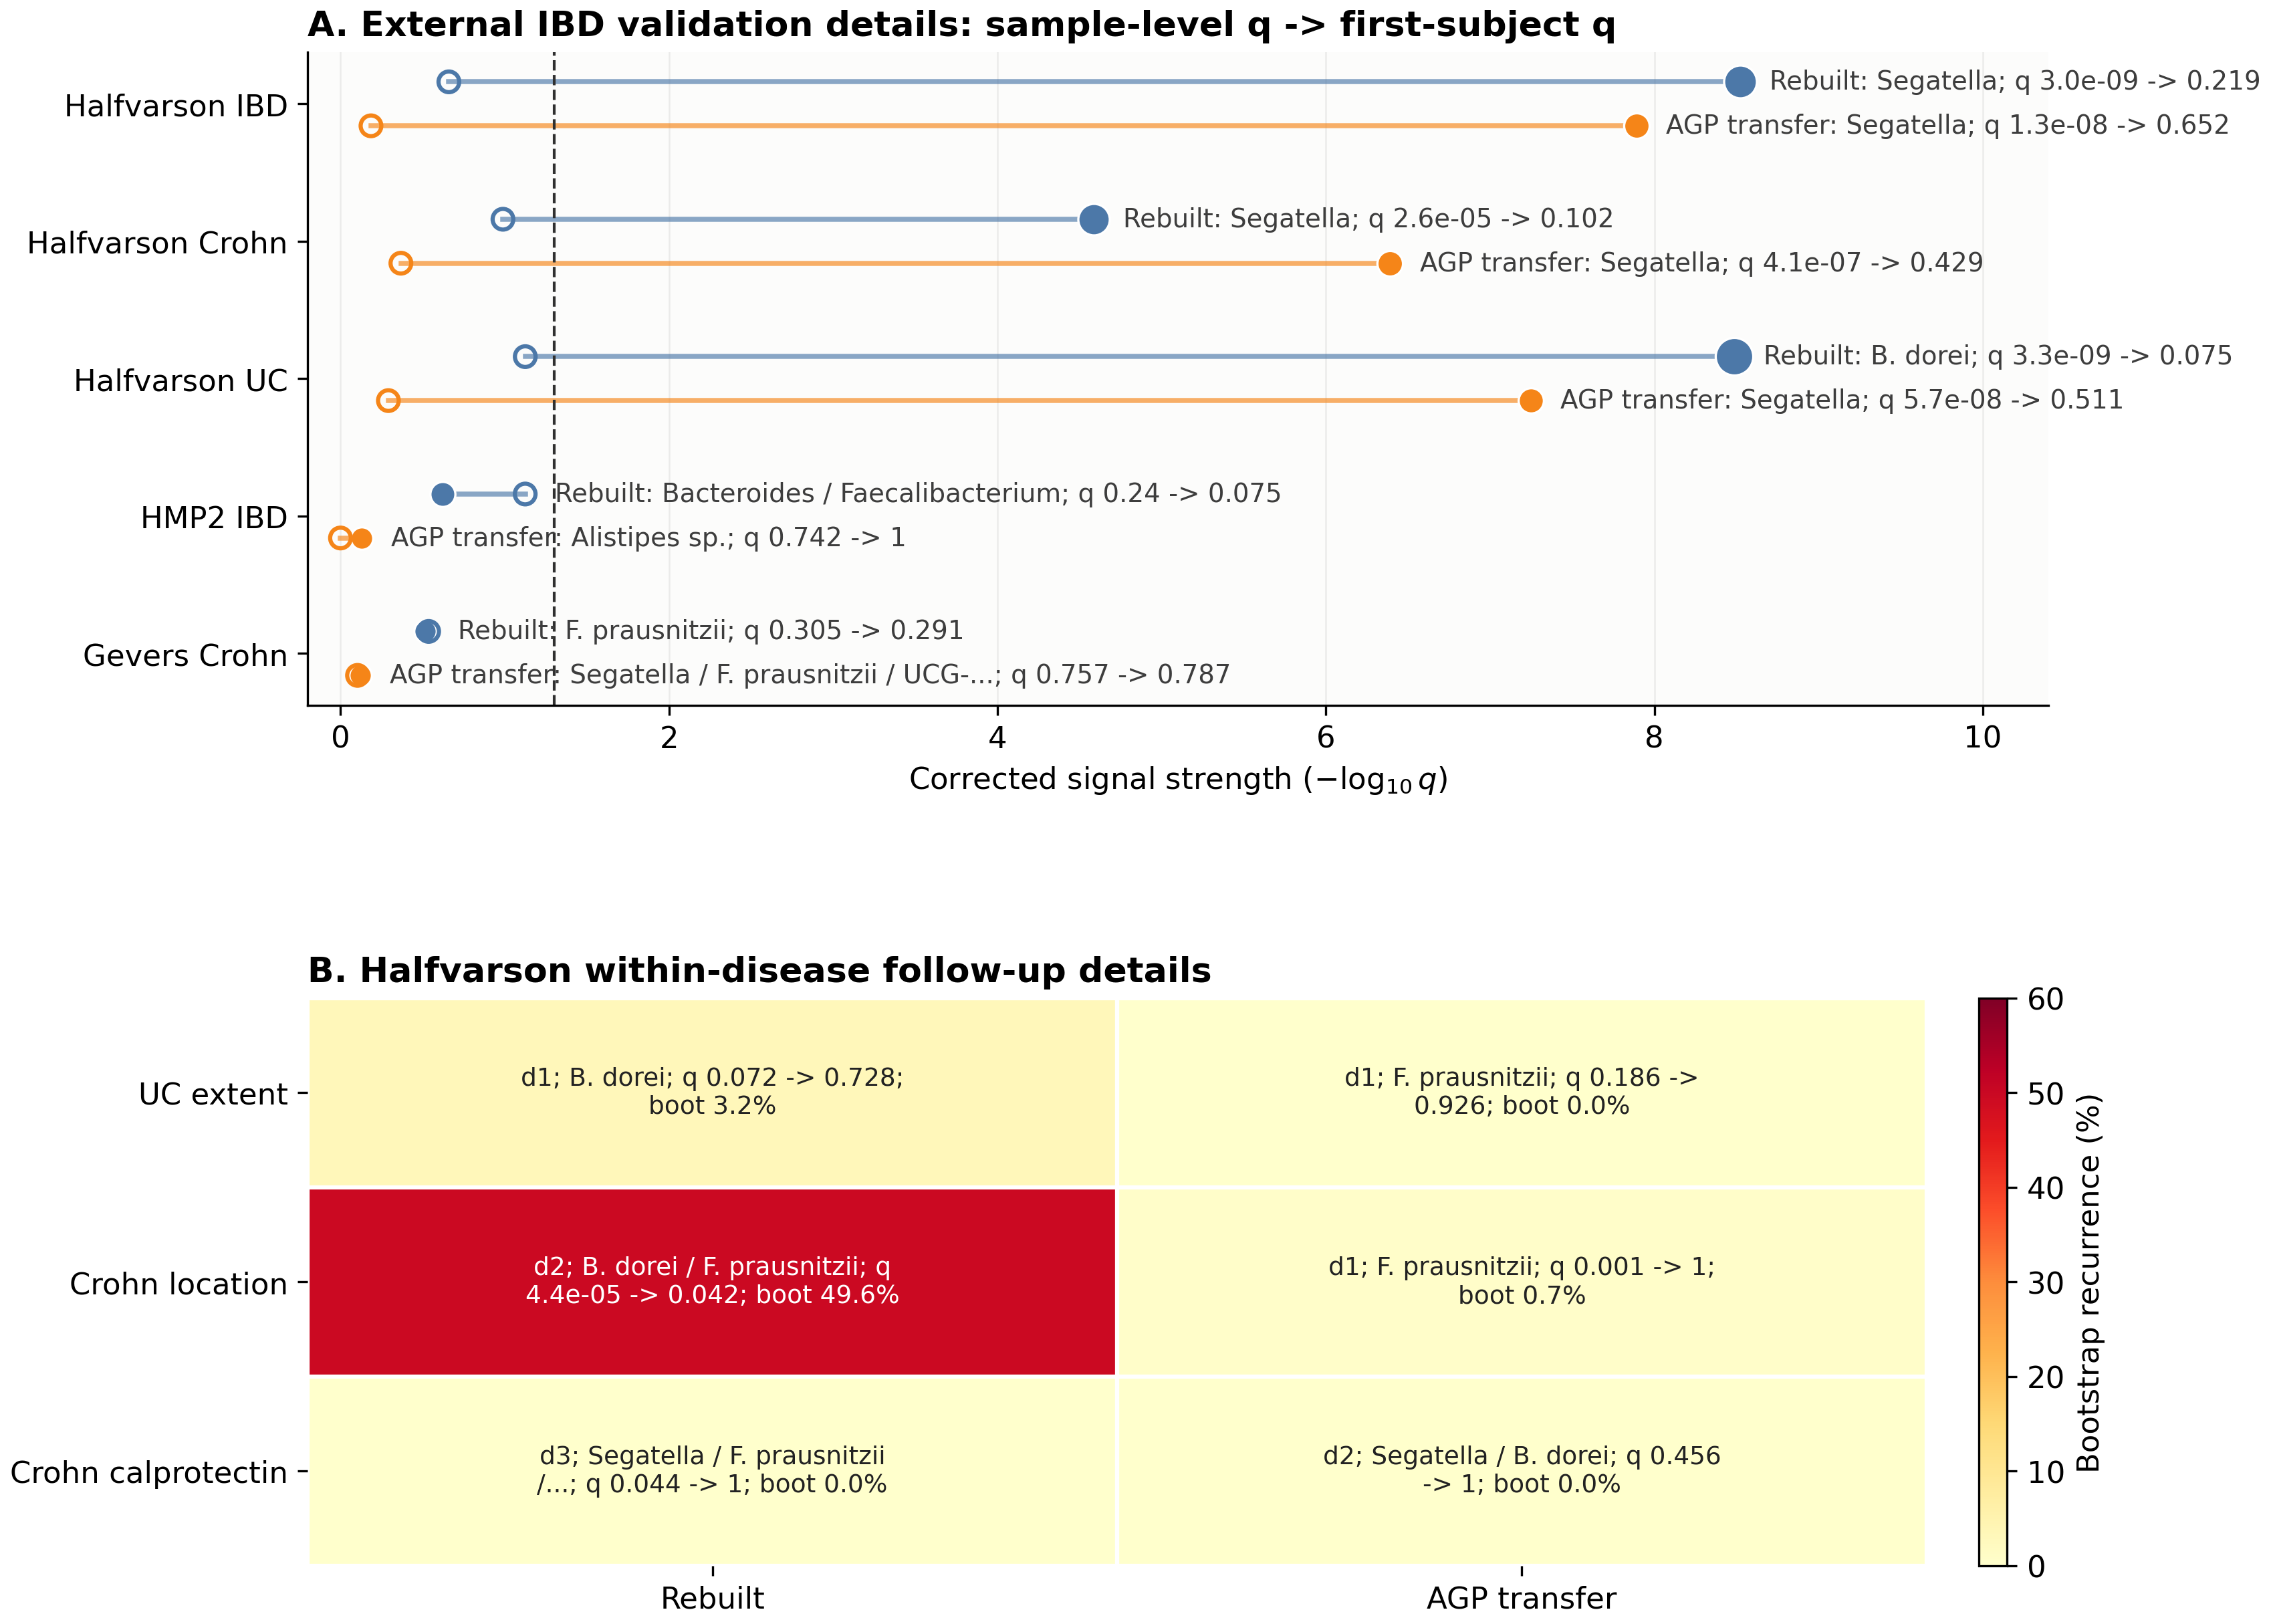
\includegraphics[width=0.98\linewidth,height=0.88\textheight,keepaspectratio]{../assets/figures/FIGURE_S1_gut_validation_detail.png}
\caption{Expanded gut validation details. Panel A shows label-level details for
the external IBD validation contrasts summarized in Figure~\ref{fig:gut-overview},
including sample-level corrected \(q\)-values and first-subject sensitivity.
Panel B shows the Halfvarson within-disease follow-up details, including the
leading label, hierarchy depth, sample-level corrected \(q\)-value,
first-subject corrected \(q\)-value, and bootstrap recurrence.}
\label{fig:supp-gut-validation-detail}
\end{figure}

\begin{figure}[!p]
\centering
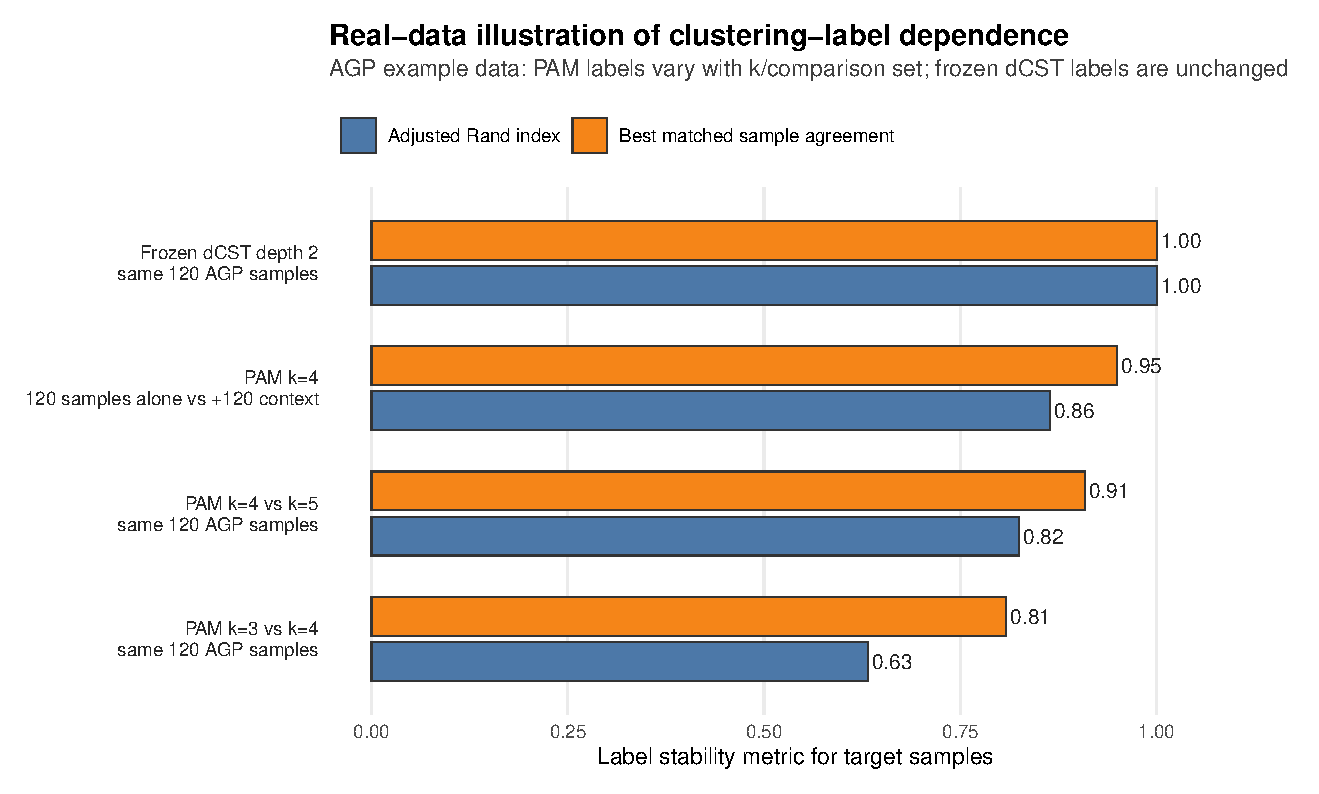
\includegraphics[width=0.98\linewidth,height=0.82\textheight,keepaspectratio]{../assets/figures/FIGURE_S2_clustering_drift_demo.pdf}
\caption{Real-data illustration of clustering-label dependence and frozen dCST
assignment. The analysis used the bundled AGP gut example matrix, with 120
target samples and 120 additional context samples selected using a fixed random
seed (20260428). PAM/enterotype-style clustering used Jensen--Shannon distance.
Label stability is summarized by the adjusted Rand index and by the best matched
sample agreement after one-to-one relabeling. The same target samples show
lower stability when \(k\) changes from 3 to 4 or 4 to 5, and when a \(k=4\)
partition is fit with or without the context samples. The frozen dCST row is
not a clustering benchmark; it shows the definitional contrast that once a
dCST hierarchy has been fitted and frozen, the same aligned target samples are
assigned to the same realized depth-2 labels without refitting.}
\label{fig:supp-clustering-contrast}
\end{figure}

\end{document}
